\documentclass{article} % For LaTeX2e
\usepackage{nips,times}
\usepackage{hyperref}
\usepackage{url}
\usepackage{enumitem}   
\usepackage{url}
\usepackage{graphicx}
\usepackage{subcaption}
\usepackage{natbib}
\usepackage{algorithm}
\usepackage{algorithmic}
\usepackage{natbib}
\usepackage{amsmath,amssymb,amsfonts,bm}
\usepackage{float}
\usepackage{booktabs} % For formal tables
\usepackage{url}
\usepackage{graphicx}
\usepackage{subcaption}
\usepackage{natbib}
\usepackage{algorithm}
\usepackage{algorithmic}
\setlength{\bibsep}{0.0pt}
\newcommand{\bX}{\mathbf{X}}
\newcommand{\bx}{\mathbf{x}}
\newcommand{\bH}{\mathbf{H}}
\newcommand{\bh}{\mathbf{h}}
\newcommand{\bY}{\mathbf{Y}}
\newcommand{\by}{\mathbf{y}}
\newcommand{\bE}{\bs{E}}
\newcommand{\bA}{\bs{A}}
\newcommand{\mL}{\mathcal{L}}
\title{Machine Learning Course Project}
\author{Zhenghui Wang, Ruijie Wang\\
	Shanghai Jiao Tong University\\
{\tt felixwzh@sjtu.edu.cn wjerry5@sjtu.edu.cn}\\
{\tt 515021910120 515021910338}
}

\newcommand{\fix}{\marginpar{FIX}}
\newcommand{\new}{\marginpar{NEW}}
\renewcommand{\algorithmicrequire}{\textbf{Input:}} 
\renewcommand{\algorithmicensure}{\textbf{Output:}}
\nipsfinalcopy

\begin{document}


\maketitle


\section{Introduction}
In this paper, we study the problem of image classification on a modified MNIST dataset with 60000 training samples and 10000 testing samples. We first use Convolutional Neural Networks as well as some data augmentation and achieve accuracy of 97.31\% for single model and 98.98 for ensemble model. Second, to handle the rotation and shifting problem, we utilize Capsule Network on the modified MNIST dataset and get much higher accuracy of 98.83\% on single model. Third, we also want to find what if we use some non-differentiable (e.g., decision tree). But traditional decision tree doesn't work well on image data, so we tend to investigate deep forest, which is a alternative of deep learning. With this deep forest, we get accuracy of 96.69\%. Last but not the least, we want study how can we train a high-performance classifier with no label information on the modified MNIST dataset. This setting is called domain adaptation. Using several SOTA domain adaptation methods, we get an accuracy of 92.51\% on the modified MNIST dataset transferring from a related USPS dataset. The code is publicly available at \url{https://github.com/felixwzh/SJTU-CS420}.
\section{Models}

\subsection{Convolutional Neural Network}
Convolutional Neural Networks (ConvNets) are a category of Neural Networks that have proven very effective in areas such as image recognition and classification. ConvNets aim to use spatial information between the pixels of an image based on discrete convolution. We follow \citep{cnn} and introduce the different types of layers used in convolutional neural networks. Based on these layers, complex architectures can be designed for image classification. 

\textbf{Convolutional Layer.} Let layer $l$ be a convolutional layer. Then, the input of layer $l$ comprises $m_1^{ (l-1) }$ feature maps from the previous layer, each of size $m_2^{(l-1)} \times m_3^{(l-1)}$. In the case where $l = 1$, the input is a single image $I$ consisting of one or more channels. This way, a convolutional neural network directly accepts raw images as input. The output of layer $l$ consists of $m_1^{(l)}$ feature maps of size $m_2^{(l)} \times m_3^{(l)}$. The $i^{th}$ feature map in layer $l$, denoted as $Y^(l)$, is computed as
\begin{equation}
Y_i^{(l)}=B_i^{(l)}+\sum^{m_{1}^{l-1}}_{j=1} K_{(i,j)}^{(l)} \star Y_{j}^{(l-1)}
\end{equation}
where $B_i^{(l)}$ is a bias matrix and $K_{(i,j)}^{(l)}$ is the filter of size $(2h^{(l)} + 1)\times (2h^{(l)} + 1)$ connecting the $j_{th}$ feature map in layer $l-1$with the $i_{th}$ feature map in layer $l$. The trainable weights of the network can be found in the filters$ K^{(l)}$ and the bias matrices $B^{(l)}$. 

\textbf{Pooling Layer.} It is common to periodically insert a Pooling layer in-between successive convolutional layers in a ConvNets architecture. Its function is to progressively reduce the spatial size of the representation to reduce the amount of parameters and computation in the network, and hence to also control overfitting. The Pooling Layer operates independently on every depth slice of the input and resizes it spatially, using the MAX operation. The most common form is a pooling layer with filters of size 2x2 applied with a stride of 2 downsamples every depth slice in the input by 2 along both width and height. 

\textbf{Fully Connected Layer.} Neurons in a fully connected layer have full connections to all activations in the previous layer, as seen in regular Neural Networks. Their activations can hence be computed with a matrix multiplication followed by a bias offset. In practice, convolutional layers are used to learn a feature hierarchy and one or more fully connected layers are used for classification purposes based on the computed features \cite{LBD89, LKF10}. 

\textbf{Architectures.} Based on the these layers, complex architectures can be designed for image classification. Figure \ref{fig:cnn_example} shows LeNet-5 as an example of ConvNets architectures.
\begin{figure}[h]
	\centering
	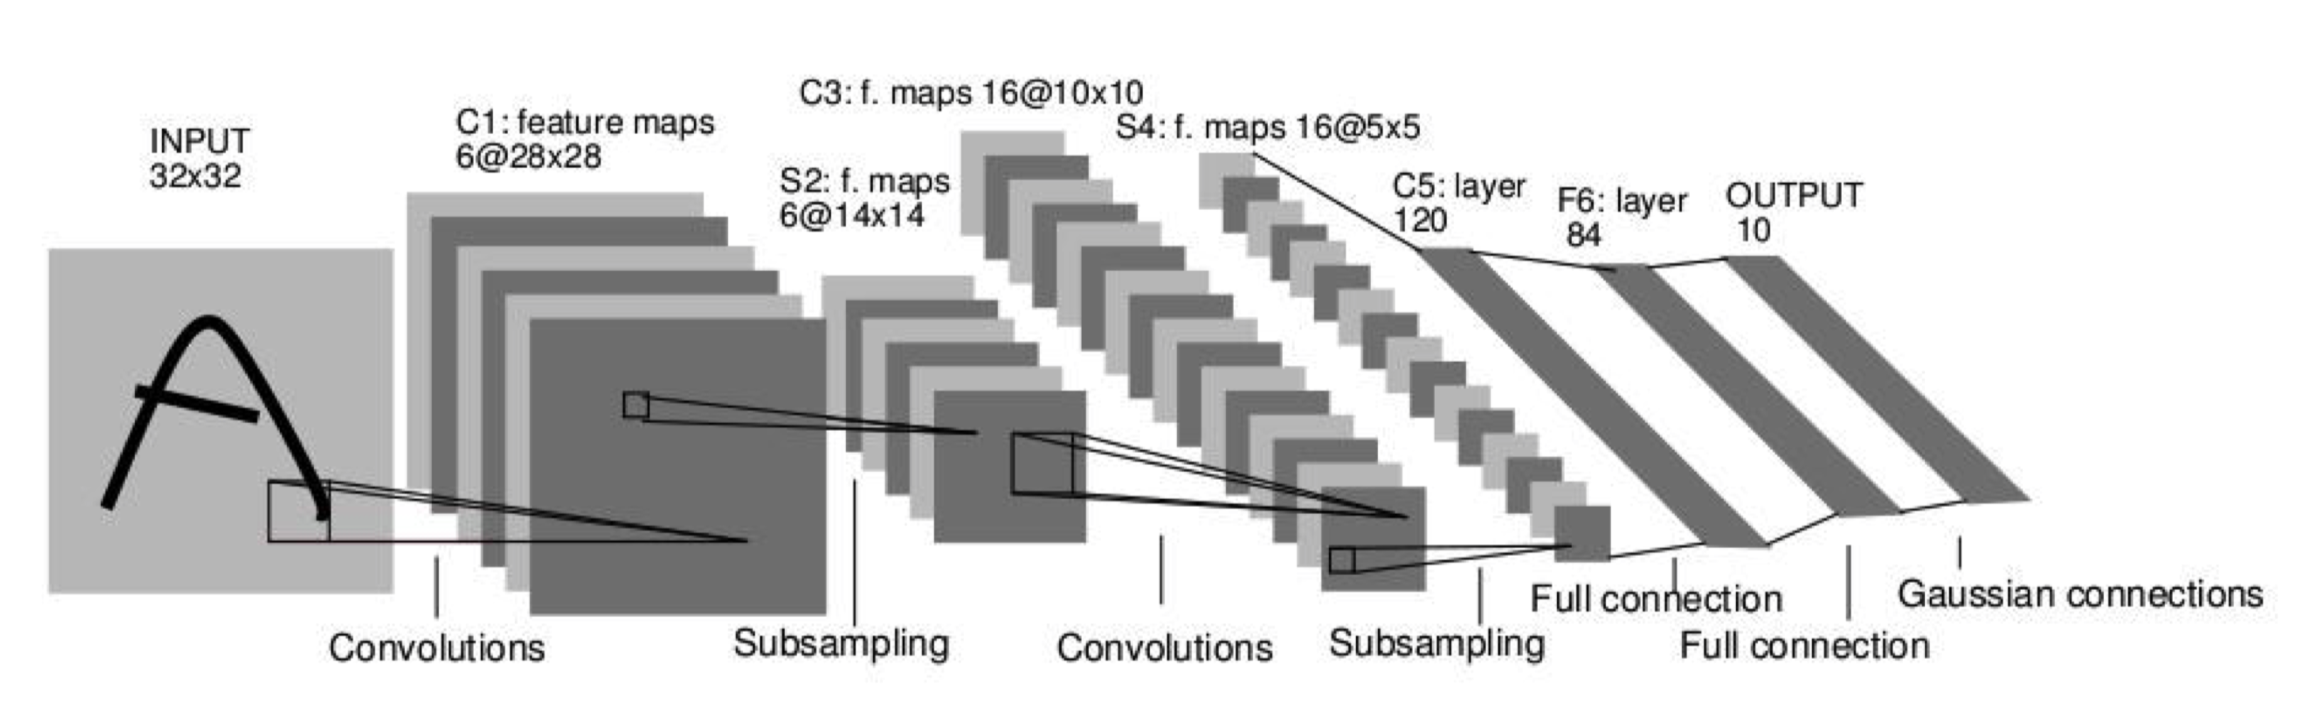
\includegraphics[width=\textwidth=0.95\widthtext]{figs/cnn_example.png}
	\caption{An example of ConvNets architectures, LeNet-5}
	\label{fig:cnn_example}
\end{figure}

\subsection{Capsule Network}
Capsule networks (CapsNets) \cite{capsnet} represent a recent breakthrough in neural network architectures.  They achieve state of the art accuracy on the MNIST dataset. CapsNets are designed based on the insights that various properties of a particular entity are presented in the image and these properties can include many different types of information. To extract those features, the  ConvNets go deeper in terms of height, while the CapsNets deepen in terms of nesting or internal structure.This idea is implemented with a capsule network contains multiple layers within a single capsule.

\textbf{Capsules.} Compared with the typical neuron which has the scalar input and output,  a capsule 
output a vector. And based on the vector output, it uses a powerful dynamic routing mechanism to ensure that the output of the capsule gets sent to an appropriate parent in the layer above. 
Figure \ref{capsule} shows the fundamental structure of capsule and the difference between the capsules and neurons . 
\begin{figure}[htbp]
	\centering
	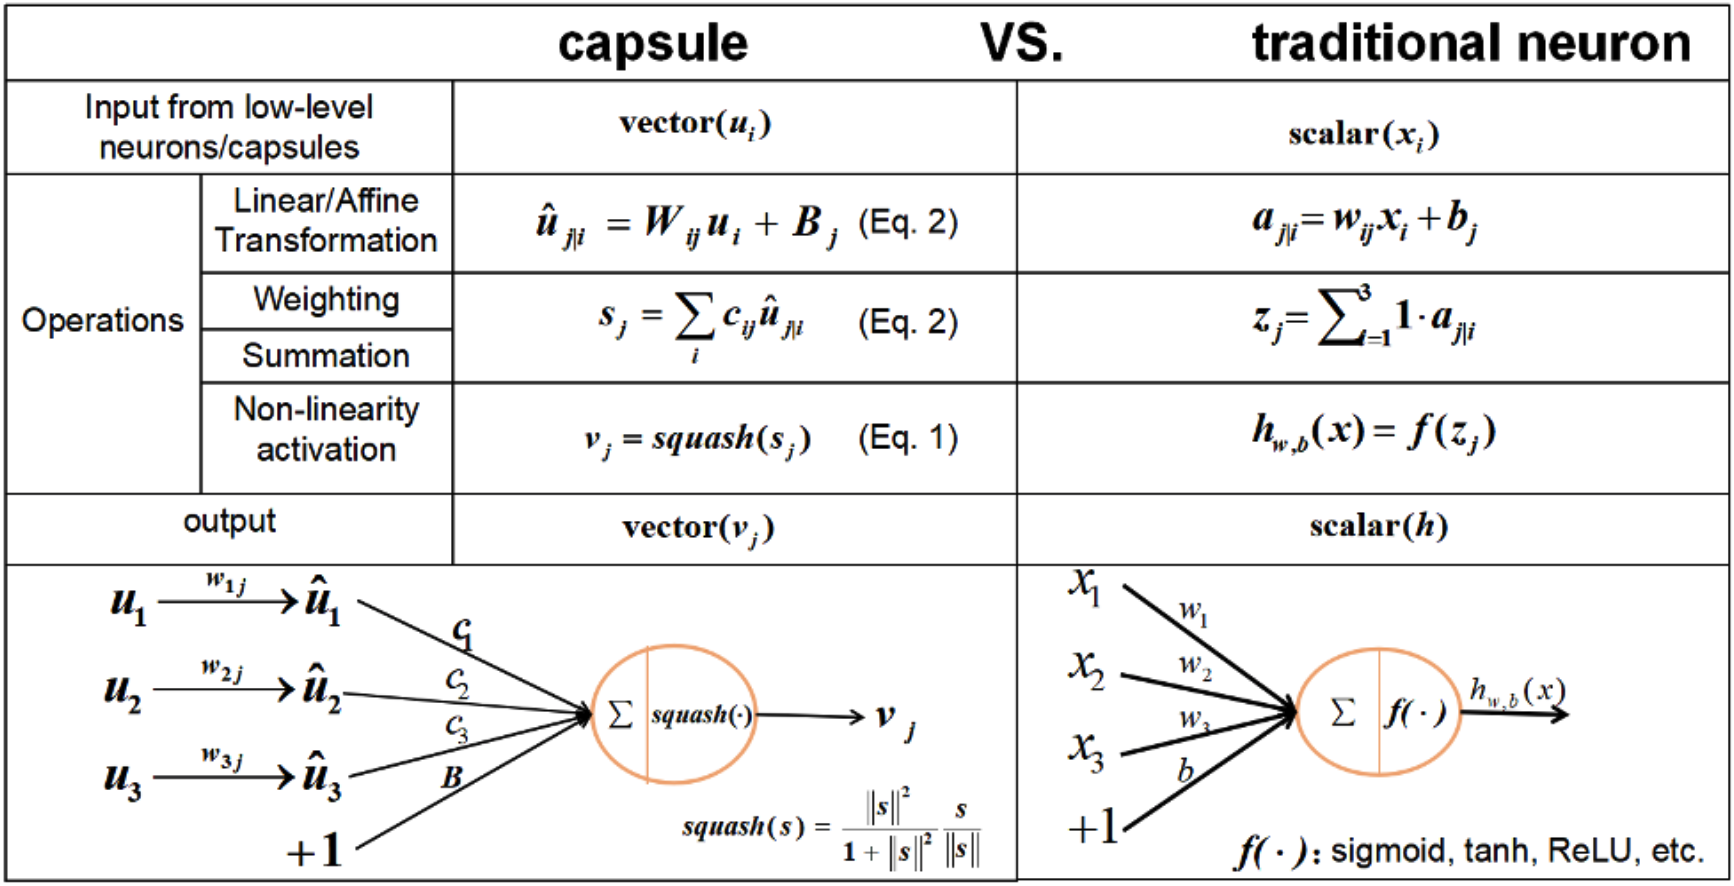
\includegraphics[width=0.7\textwidth]{figs/capsule.png}
	\caption{The difference between capsule and neurons. The neuron has a scalar input and output, while capsule has a vector input and output. Therefore a special squash operation is designed to conduct non-linear activation.}
	\label{capsule}
\end{figure}

As it shown in \ref{capsule}, $\vec{v}$ and $\hat{\vec{u}}$ denote the input and output of a capsule. While receiving the output $\vec{u}$ from the layer below,  $\hat{\vec{u}}$ is produced by multiplying $\vec{u_i}$ by a weight matrix $\vec{W}_{ij}$. To calculate the output of a capsule, non-linear squashing is used, which makes sure that the length of the output vector of a capsule to represent the probability that the entity represented by the capsule is present in the current input. The coupling coefficients between capsule $i$ and all the capsules in the layer above sum to $1$ and are determined by a ¡°routing softmax¡± whose initial logits $b_{ij}$ are the log prior probabilities that capsule $i$ should be coupled to capsule $j$. 
\begin{equation}
c_{ij}=\frac{exp(b_{ij})}{\sum_{k}exp(b_{ik})}
\end{equation}
\textbf{Margin loss for digit existence.} If digit $k$ is present in the image, the expected result is that  the top-level capsule for digit class k to have a long instantiation vector. The margin loss is defined in Eq. \ref{eq:margin}.
\begin{equation}
L_K=T_k \space \max (0, m^+ - \| \vec{v_k}\| )^2 + \lambda(1-T_k) \space \max (0,\| \vec{v_k}\| - m^-)^2
\label{eq:margin}
\end{equation}
where $T_k=1$ iff a digit of class k is present.

\textbf{CapsNet architecture.} The architecture is shallow with only two convolutional layers and one fully connected layer. Conv1 converts pixel intensities to the activities of local feature detectors that are then used as inputs to the following primary capsules. The second layer (PrimaryCapsules) is a convolutional capsule layer with 32 channels of convolutional 8D capsules. The final Layer (DigitCaps) has one 16D capsule per digit class and each of these capsules receives input from all the capsules in the layer below. And the model only apply routing algorithm between PrimaryCapsules and DigitCaps. The  architecture is shown in Figure \ref{fig:capsnet}.
\begin{figure}[htbp]
	\centering
	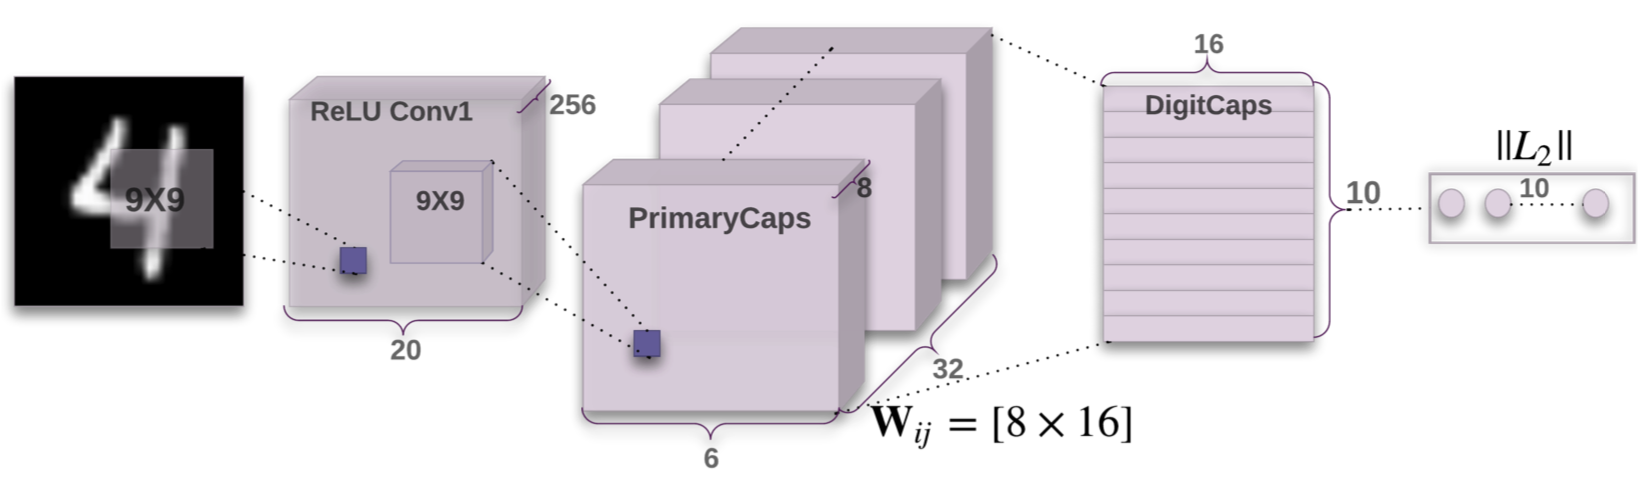
\includegraphics[width=0.9\textwidth]{figs/capsnet.png}
	\caption{The architecture of CapsNet.}
	\label{fig:capsnet}
\end{figure}

\textbf{Reconstruction.} A additional reconstruction loss is designed to  use this activity vector to reconstruct the input image. The decoder is consisting of 3 fully connected layers, which is shown in Figure \ref{fig:reconstruction}.
\begin{figure}[htbp]
	\centering
	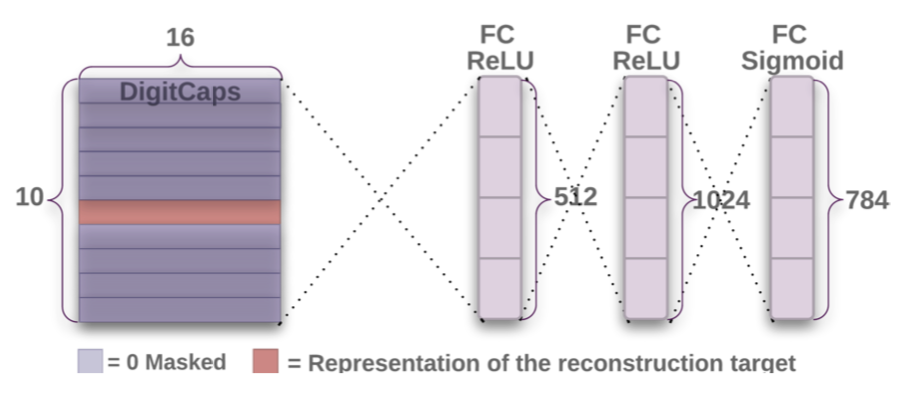
\includegraphics[width=0.9\textwidth]{figs/construction.png}
	\caption{The architecture of CapsNet.}
	\label{fig:reconstruction}
\end{figure}

\subsection{Deep Forest}
Deep forest (DF) is a decision tree ensemble approach with highly competitive performance to deep neural networks. It is recently proposed by \cite{zhou2017deep}. It is well known that when we talk about the term \textit{deep}, we usually mean many layers of neural networks such as the very deep convolutional neural networks' variant -- ResNet \cite{he2016deep} or the deep recurrent neural networks in temporal sequence like long short-term memory (LSTM) \cite{hochreiter1997long}. We rarely construct some kind of \textit{deep} model for traditional models, especially for those models which do not use a gradient based learning approach like random forest.

However, \cite{zhou2017deep} successfully construct a multi-layer ensemble approach using traditional models -- random forest. More specificly, deep forest use so-called multi-grained sacnning (illustrated in Figure~\ref{fig:multi-grained-scanning}) to do representation learning. It is similar to the convolution operation but with a decision tree based approach. 
\begin{figure}[h]
	\centering
	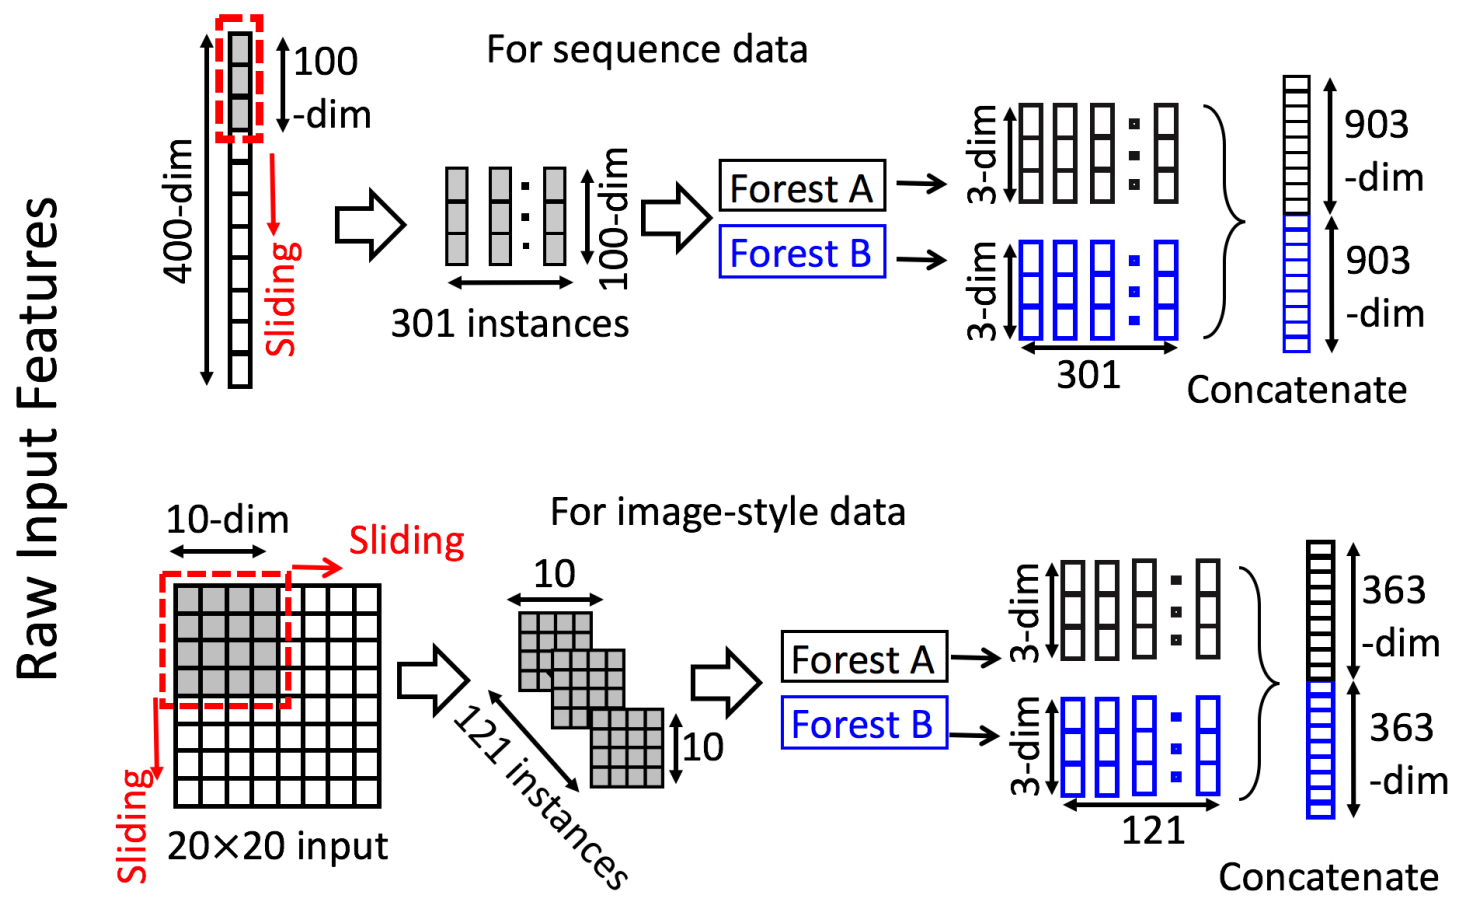
\includegraphics[width=0.7\linewidth]{./figs/multi-grained-scanning}
	\caption{ Illustration of feature re-representation using multi-grained sacnning. Suppose there are three classes, raw features are 400-dim, and sliding window is 100-dim.}
	\label{fig:multi-grained-scanning}
\end{figure}

After the multi-grained sacnning layer, a cascade forest structure is leveraged to learn better representation in a level-by-level way. Each level is an ensemble fo decision tree forest. And the \textit{diversity} is encouraged by incluing different types of forest like 2 random forests with $k=\sqrt{d}$ and 2 completely-random tree forests with $k=1$. The split is guided by the \textit{gini} value. The construction of the levels are adaptive. Each level will generate a class vector as a leared representation for next level and each level's input are the origin feature vector concatenated with early level's output class vector. For each level, we evaluate the performance with $k$-fold cross validation. If there is no significant improvement of the performance, we stop the training. The illustration for both multi-grained sacnning and cascade forest structure are shown in Figure~\ref{fig:deep-forest}, which is the whole model's pipline. 



\begin{figure*}[h]
	\centering
	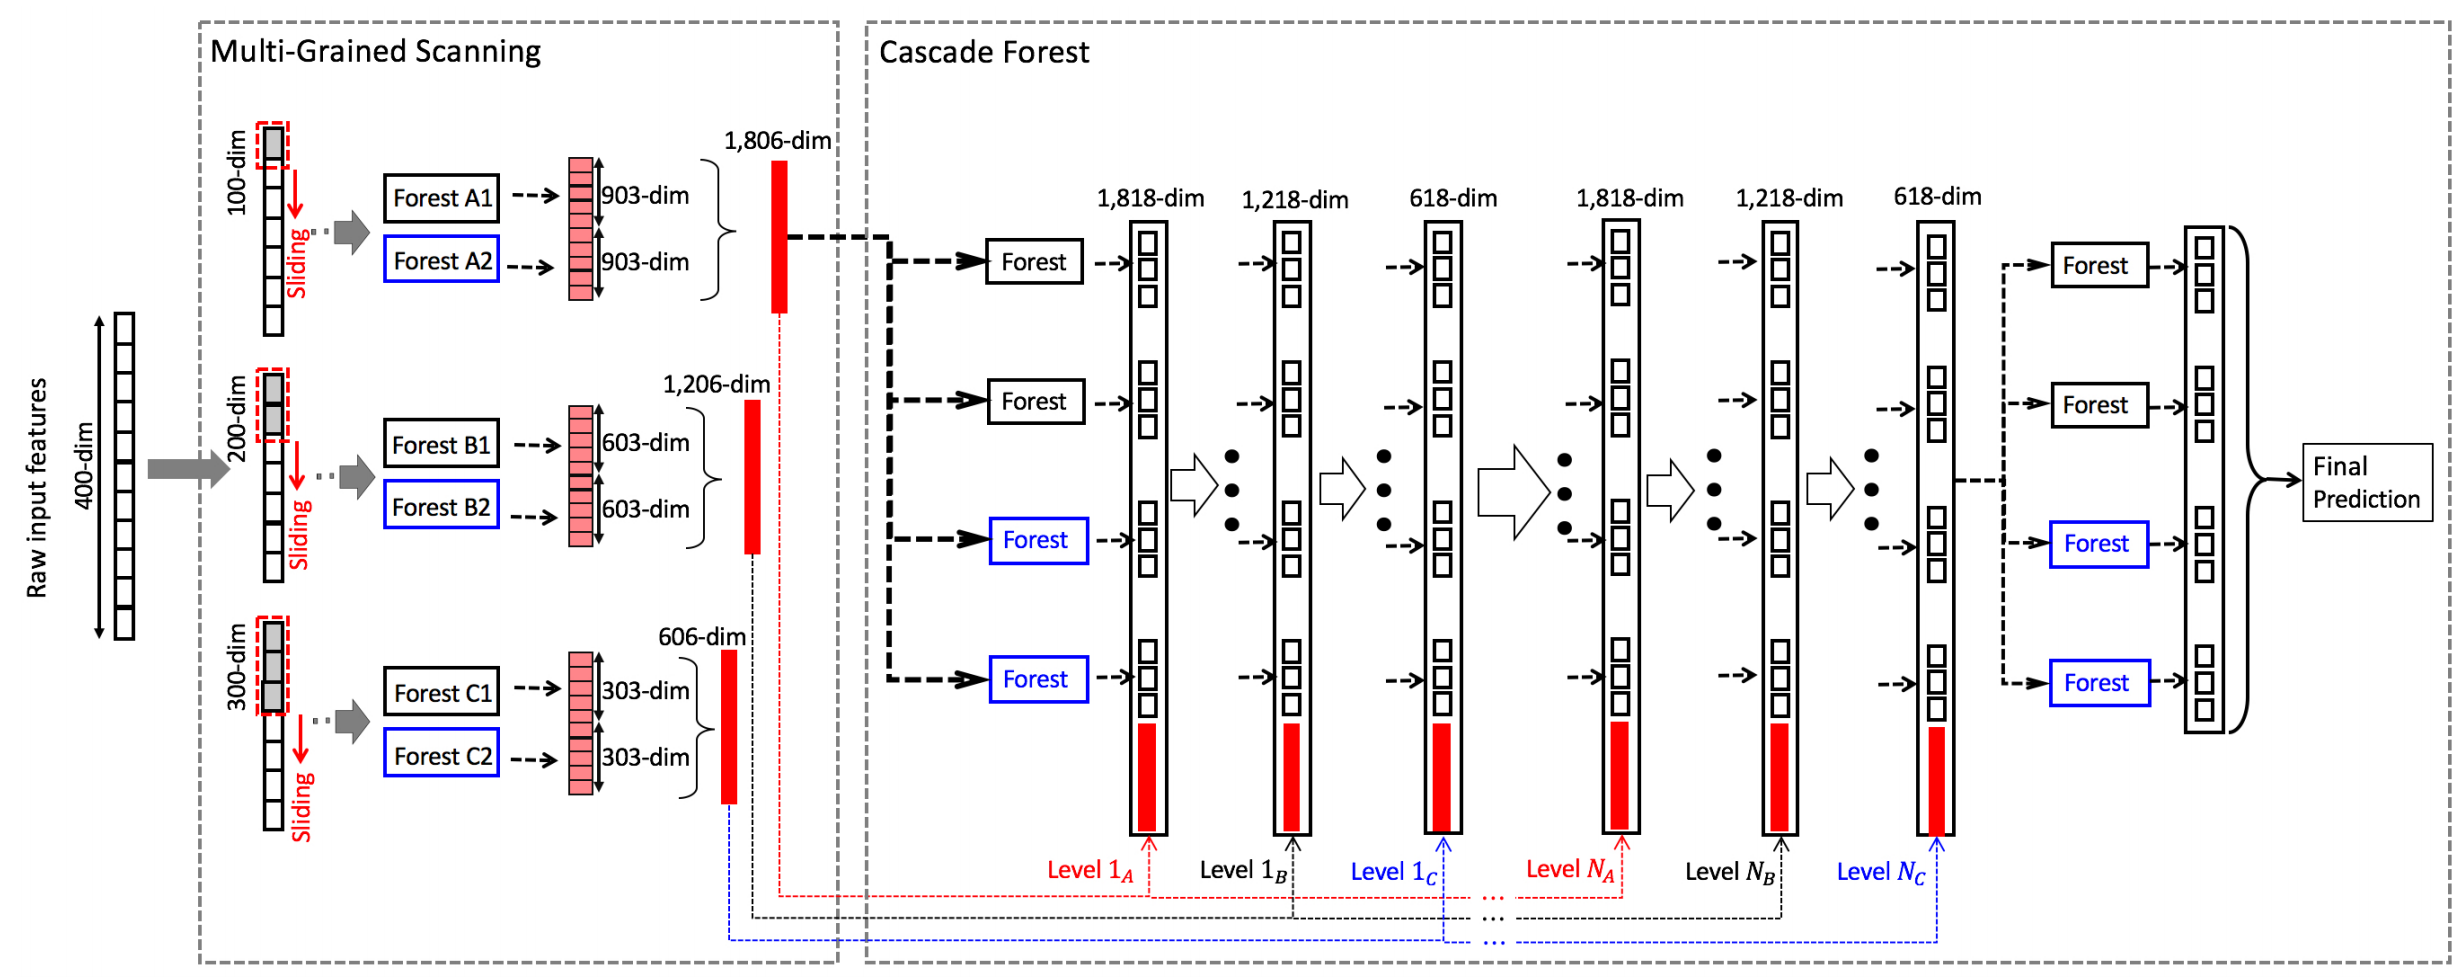
\includegraphics[width=1\linewidth]{./figs/deep-forest}
	\caption{The overall procedure of deep forest. Suppose there are three classes to predict, raw features are 400-dim, and three sizes of sliding windows are used.}
	\label{fig:deep-forest}
\end{figure*}

\subsection{Domain Adaptation}
In this paper, we want to study if we have data from another domain, how well can we learn a classifier on the MNIST dataset with no label information. Thus domain adaptation is a very suitable learning scenario for this purpose.

Domain adaptation is a subtask of transfer learning which aims at generalizing a high-performance learner on a target domain via utilizing the knowledge distilled from a source domain which has a different but related data distribution. Note that for in domain adaptation scenario, we only have labeled data on source domain but unlabeled data on target domain. One solution to domain adaptation is to learn domain invariant feature representations while the learned representations should also be discriminative in prediction. To learn such representations, domain adaptation frameworks usually include a domain invariant representation learning approach to measure and reduce the domain discrepancy, as well as a discriminator for classification. 

Several methods have been proposed for `deep' models in thsi deep learning era. We briefly introduce MMD \cite{long2015learning}, CORAL \cite{sun2016return}, DANN \cite{ajakan2014domain,ganin2016domain}, WDGRL \cite{shen2017adversarial}, which are all state-of-the-art doamin adaptation methods. 

Deep adaptation network (DAN) \cite{long2015learning} was proposed to enhance the feature transferability by minimizing multi-kernel MMD in several task-specific layers (architecture shown in Figure~\ref{fig:mmd}). The squared formulation of MK-MMD is defined as
\begin{equation}\label{eqn:MMD}
d_k^2\left( {p,q} \right) \triangleq \left\| {{{\mathbf{E}}_p}\left[ {\phi \left( {{{\mathbf{x}}^s}} \right)} \right] - {{\mathbf{E}}_q}\left[ {\phi \left( {{{\mathbf{x}}^t}} \right)} \right]} \right\|_{{\mathcal{H}_k}}^2.
\end{equation}
And in DAN it reduce the MK-MMD of hidden representations between source and target domain as shown in Figure~\ref{fig:mmd}
\begin{figure}[H]
\centering
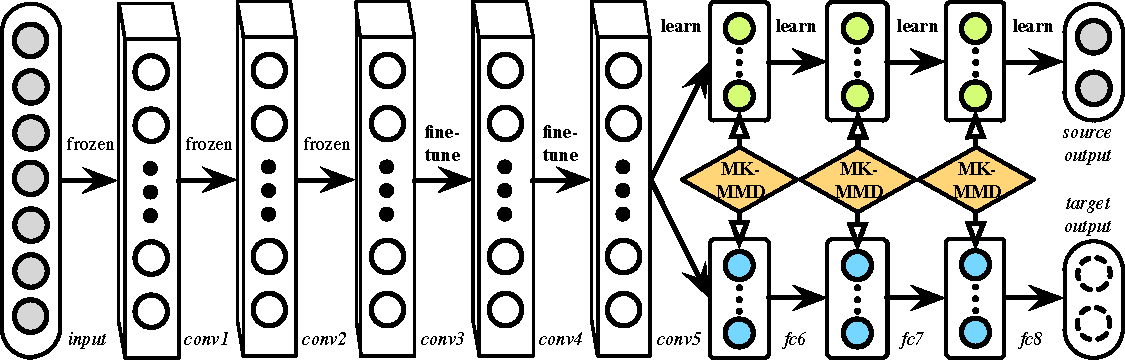
\includegraphics[width=0.7\linewidth]{figs/DAN}
\caption{Illustration of MMD method.}
\label{fig:mmd}
\end{figure}



On the other hand, correlation alignment (CORAL) method \cite{sun2016return} was proposed to align the second-order statistics of the source and target distributions with a linear transformation and the illustration can be found in Figure~\ref{fig:coral}.
\begin{figure}[H]
	\centering
	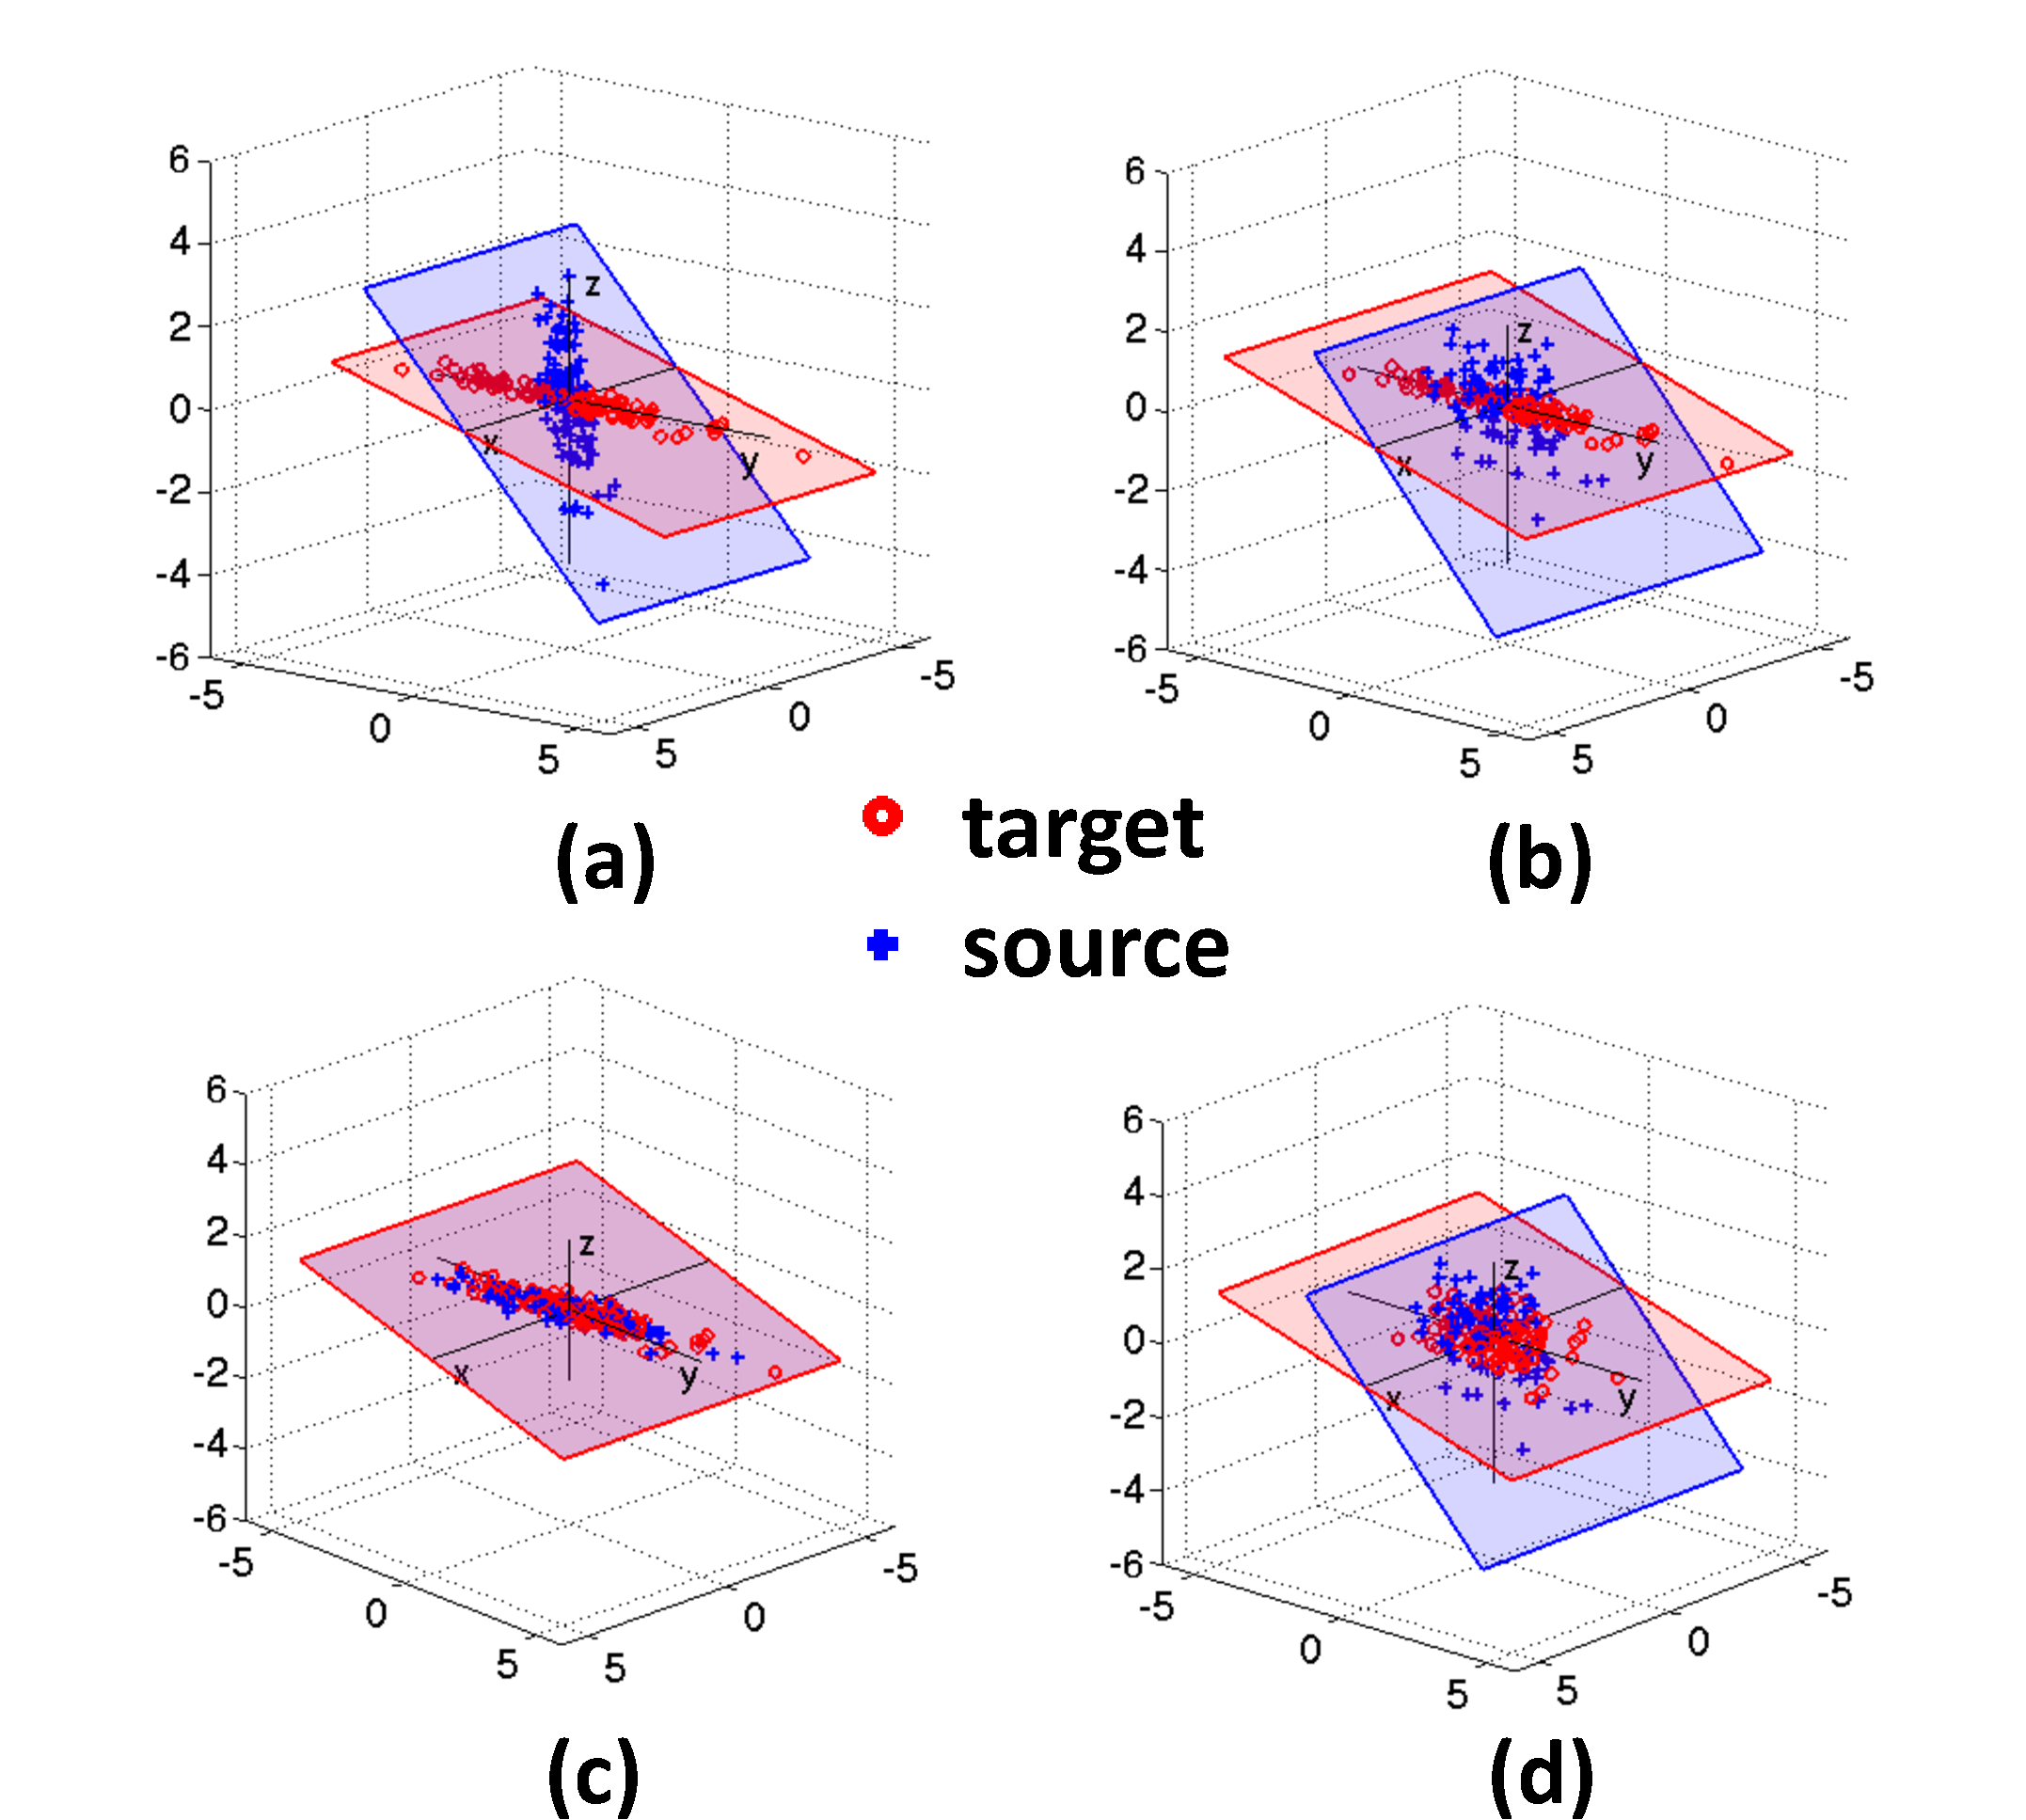
\includegraphics[width=0.7\linewidth]{figs/coral}
	\caption{\small \textbf{(a-c)} Illustration of CORrelation ALignment (CORAL) for Domain Adaptation: (a) The original source and target domains have different distribution covariances, despite the features being normalized to zero mean and unit standard deviation. This presents a problem for transferring classifiers trained on source to target. (b) The same two domains after source decorrelation, i.e. removing the feature correlations of the source domain. (c) Target re-correlation, adding the correlation of the target domain to the source features. After this step, the source and target distributions are well aligned and the classifier trained on the adjusted source domain is expected to work well in the target domain. \textbf{(d)} One might instead attempt to align the distributions by whitening both source and target. However, this will fail since the source and target data are likely to lie on different subspaces due to domain shift.}
	\label{fig:coral}
\end{figure}

Motivated by theory in \cite{ben2007analysis,ben2010theory} suggesting that a good cross-domain representation contains no discriminative information about the origin (i.e. domain) of the input, domain adversarial neural network (DANN) \cite{ajakan2014domain,ganin2016domain} was proposed to learn domain invariant features by a minimax game between the domain classifier and the feature extractor (shown in Figure~\ref{fig:DANN}). 
\begin{figure}[H]
\centering
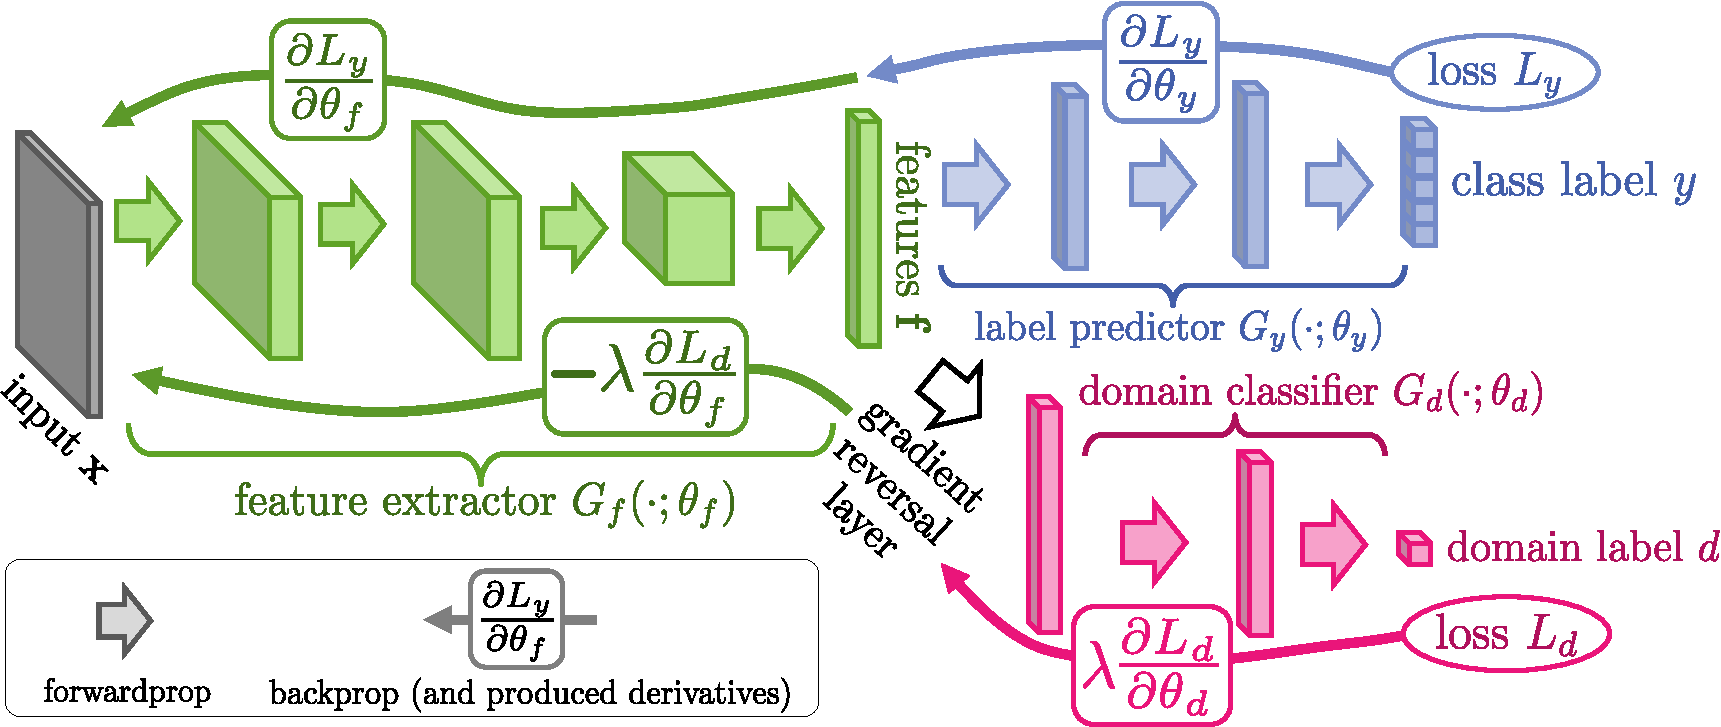
\includegraphics[width=0.7\linewidth]{figs/DANN}
\caption{Illustration of DANN.}
\label{fig:DANN}
\end{figure}

Wasserstein Distance Guided Representation Learning (WDGRL) \cite{shen2017adversarial} utilizes a neural network, denoted by the domain critic, to estimate empirical Wasserstein distance between the source and target samples and optimizes the feature extractor network to minimize the estimated Wasserstein distance in an adversarial manner. The illustration of WDGRL is shown in Figure~\ref{fig:wd}.

\begin{figure}[H]
\centering
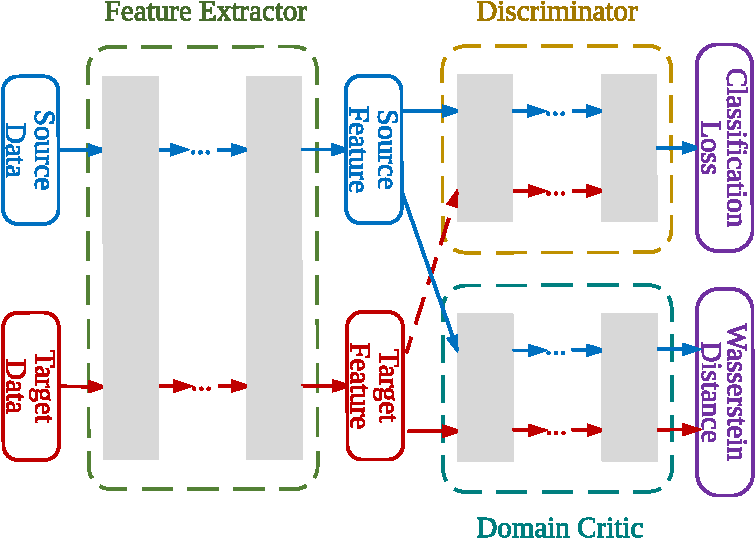
\includegraphics[width=0.7\linewidth]{figs/wd}
\caption{illustration of WDGRL.}
\label{fig:wd}
\end{figure}


In this paper, we adopted all the aforementioned methods to conduct domain adaptation in our MNIST dataset. The source domain is USPS dataset \cite{proedrou2002transductive}. The dataset refers to numeric data obtained from the scanning of handwritten digits from envelopes by the U.S. Postal Service. The original scanned digits are binary and of different sizes and orientations; the images here have been deslanted and size normalized, resulting in 16 x 16 grayscale images. The USPS dataset is similar but not identical to MNIST dataset, which can be figured out in the comparison in Figure~\ref{fig:usps-mnist}. But as the size of the given MNIST dataset for this project is 45 x 45, we pad the image in USPS randomly and get the same 45 x 45 size. Then we use all the training data with label in USPS but data in MNIST with out data to train a classifier. Thus the USPS is the \textit{source domain} while MNIST is the \textit{target domain}.

\begin{figure}[H]
\centering
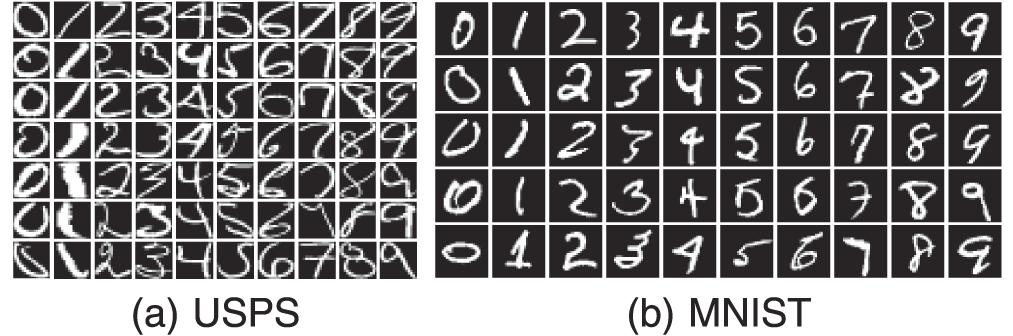
\includegraphics[width=0.7\linewidth]{figs/usps-mnist}
\caption{Comparison of USPS and MNIST datas/et.}
\label{fig:usps-mnist}
\end{figure}

\section{Experiments}
\subsection{ConvNets}
Figure \ref{fig:excnn} shows the structure of ConvNets we use. 
\begin{figure}[htbp]
	\centering
	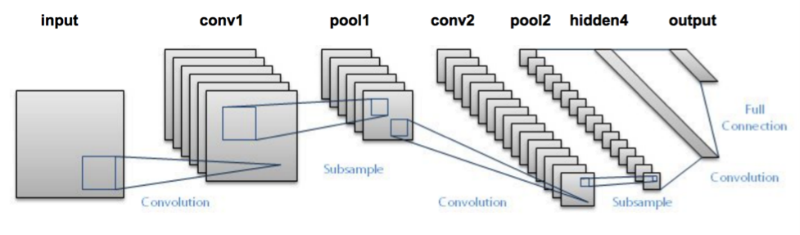
\includegraphics[width=0.9\textwidth]{figs/cnn.png}
	\caption{The architecture of experiment ConvNets, which consists of $5\times5$ convlution, $2\times2$ max pooling, $5\times5$ convlution, $2\times2$ max pooling, 1024 fully connected layer,  ReLU activations, Adam optimizer, dropout.}
	\label{fig:excnn}
\end{figure}
Figure \ref{fig:process} shows the training process. The best accuracy result of single model is 97.31\%. Compared with the reported results on $25\times25$ MNIST, the lower accuracy result illustrates that the noise in image and digits movements influent the performance of ConvNets. 
\begin{figure}[htbp]
	\centering
	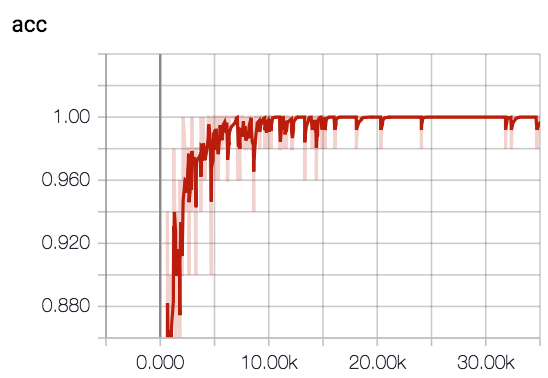
\includegraphics[width=0.3\textwidth]{figs/acc.png}
	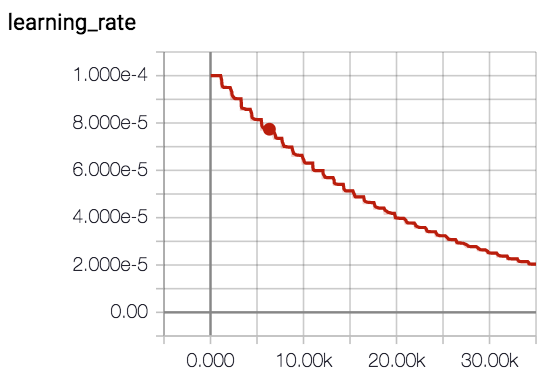
\includegraphics[width=0.3\textwidth]{figs/lr.png}
	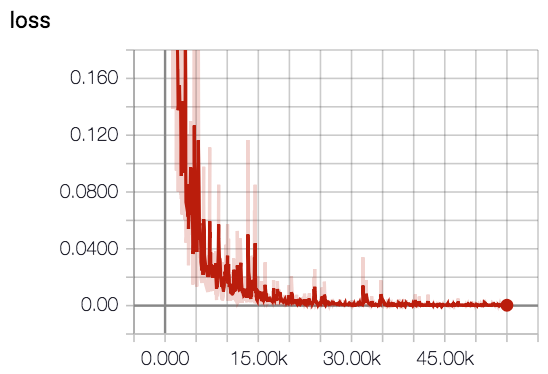
\includegraphics[width=0.3\textwidth]{figs/loss.png}
	\caption{Training process. Accuracy, learning rate, loss are reproted}
	\label{fig:process}
\end{figure}

To further improve the ConvNets performance, data augmentation and model ensemble are applied.
\begin{itemize}
	\item \textbf{Data augmentation.}  Each image is rotated by random degree in ranging [$-30^{\circ}$, $+30^{\circ}$],  and is randomly shifted by a value ranging [-10pix, +10pix] at both axises. Training data can be increased to enhance the generalization ability of the model. On the other hand, noise data can be added to enhance the robustness of the model. The best result after augmentation is up to 98.73\%, which achieve a significant improvement by 1.42\%.
	\item \textbf{Model ensemble.} We use 10 single ConvNets makes a prediction (votes) for each test instance and the final output prediction is the one that receives the highest number of votes. The best result after augmentation is 98.98\% without data augmentation, achieving a 1.67\% improment.
\end{itemize}

\subsection{CapsNets }
We explore CapsNets in \cite{capsnet} directly on the modified MNIST dataset, and no other data augmentation/deformation is used. Table \ref{tb:capsulresult} reports the test accuracy on our MNIST dataser for different CapsNet setups and shows the importance of routing and reconstruction regularizer.
\begin{table}[htbp]
	\centering
	\caption{The best result of digit classification based on CapsNet}
	\label{tb:capsulresult}
	\begin{tabular}{ccccccc}
		\hline
		Method & Routing & Reconstruction & MNIST (\%) & in paper (\%) & comparison (\%) & in paper (\%)\\
		\hline
		Baseline & - & - & 97.74 & 99.61 & 0.00 & 0.00\\
		CapsNet & 1 & 0.0 / no & 98.75 & 99.66 & +1.03 & +0.05\\
		CapsNet & 1 & 0.392 / yse & 98.76 & 99.71 &+1.02 & +0.10 \\
		CapsNet & 3 & 0.0 / no & 98.73 & 99.65 & +1.03 & +0.04\\
		CapsNet & 3 & 0.392 / yse & 98.83 & 99.75 & +1.15 & +0.14\\
		\hline
	\end{tabular}
\end{table}

The baseline is a standard CNN with three convolutional layers of 256, 256, 128 channels. Each has 5x5 kernels and stride of 1. The last convolutional layers are followed by two fully connected layers of size 328, 192. The last fully connected layer is connected with dropout to a 10 class softmax layer with cross entropy loss. All the CapsNets outperform baseline network,  and the performance gap between CapsNet and baseline is more pronounced than the result reported in \cite{capsnet}. We view it as a consequence of the way to modify the MNIST (etc. adding noises to origin image and shifting the digits). The added noises and shifted pixel enhance the advantages of capsule over typical neuron. On the other hand, the results also shows the importance of routing and reconstruction regularizer. The former algorithm can lead to a better representation of image and the latter tool helps to enhance the robustness of the model. 

We also explore the reconstruction process of the model. Figure \ref{fig:reconstruction} shows the reconstruction results.
\begin{figure}[h]
	\centering
	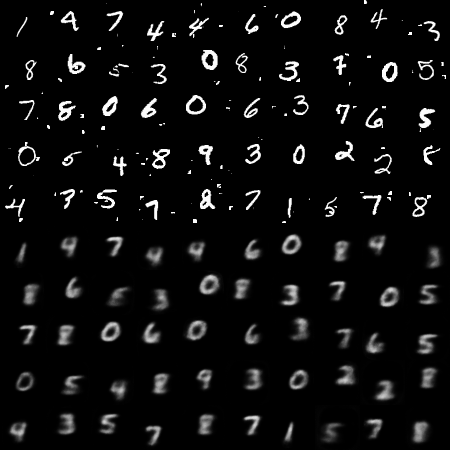
\includegraphics[width=0.7\textwidth]{figs/reconstruction.png}
	\caption{The reconstruction result on CapsNets with 3 Routing literation and 0.392 reconstruction loss coefficient. The images above are original samples and the images below are the reconstruction results. The reconstruction results filter the noise in the original image effectively. At the same time, it can be found that the reconstruction process handles the digital rotation angle in the original image very well. All of this illustrate the capsule can learn a valid representation of the original input.}
	\label{fig:reconstruction}
\end{figure}

Another interesting exploration is that what the individual dimensions of a capsule represent. We try to see what the individual dimensions represent by making use of the decoder network. Examples are shown in figure \ref{fig:newdigit}.

\begin{figure}[htbp]
	\centering
	\begin{subfigure}[b]{0.9\textwidth}
		\centering
		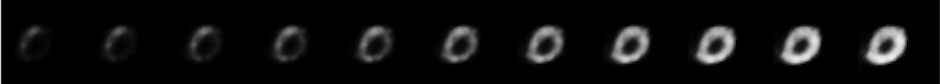
\includegraphics[width=0.9\textwidth]{figs/0.png}
		\caption{Stroke thickness represented by one dimension}
	\end{subfigure}
	\begin{subfigure}[b]{0.9\textwidth}
		\centering
		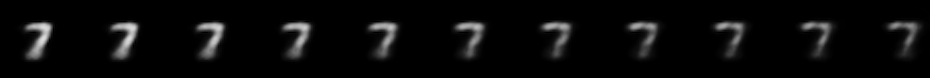
\includegraphics[width=0.9\textwidth]{figs/7.png}
		\caption{Localized part represented by one dimension}
	\end{subfigure}
	\caption{Example representation of capsule single dimension.}
	\label{fig:newdigit}
\end{figure}

\subsection{Deep Forest}
As we mentioned before, deep forest could be cascaded forest (CA) or cascaded forest with multi-grained scanning (GC). We use both this two configuration. For CA both there are a random forest with 1000 decision trees and 1000 extreme random decision trees. For GC, except the same configuration at each level, we adopt 3 fine-grained scanning with window size 7 x 7, 10 x 10 and 13 x 13.

The results are shown in Table~\ref{tab:deep-forest}. We can find that deep forest can achieve competitive performance with the cascade structure and multi-grained scanning. And the multi-grained scanning can boost the performance of cascade structure on this image classification task.
	\begin{table}[h]
		\centering
		\begin{tabular}{l|cc}
			\toprule
			Configuration&CA&GC\\
			\midrule
			Acc&92.77&\textbf{96.68}\\
			
			\bottomrule	
		\end{tabular}
		\caption{Accuracy of deep forest on MNIST with different configuration. }
		\label{tab:deep-forest}
	\end{table}

Recall that deep forest is trained layer by layer, so what is the influence of layer for deep forest? We plot the performance curve on test set for both CA and GC in Figure~\ref{fig:DF-ca-gc}. We can find that the performance improves layer by layer, especially in the first 4 layers. And then the performance converges.
\begin{figure}[h]
\centering
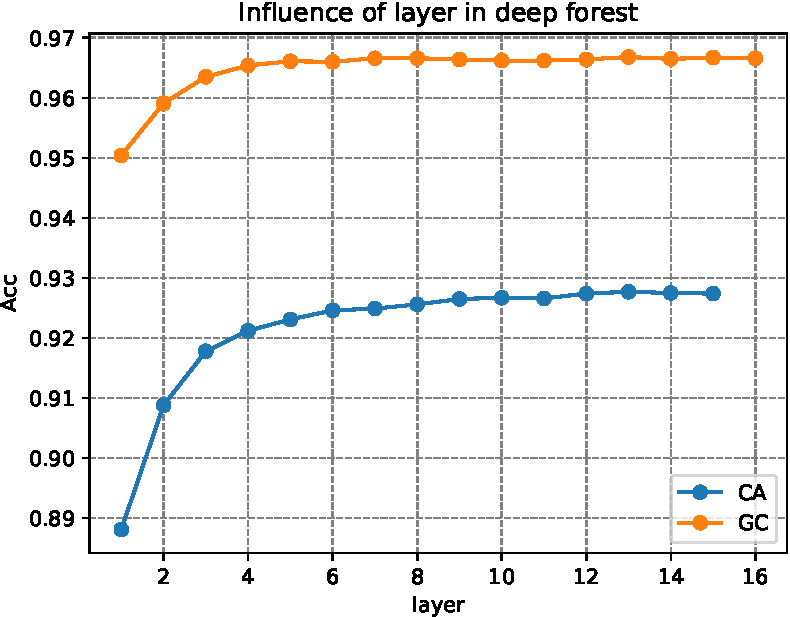
\includegraphics[width=0.7\linewidth]{figs/DF-ca-gc}
\caption{performance curve on test set for both CA and GC deep forest.}
\label{fig:DF-ca-gc}
\end{figure}



\subsection{Domain Adaptation}
For domain adaptation, we use a simple CNN for all the methods we used. The CNN has two convolutional layer with 5 x 5 kernels, two max pooling layer, and one fully connected layer. We use this simple CNN for simplicity and efficiency. CNN with more complicated architecture could also be used for domain adaptation. 
 
There are 5 methods we used for our domain adaptation experiment: S(ource)-only (only train on source domain), and MMD, CORAL, DANN, WDGRL. The overall results are shown in Table~\ref{tab:domain-adaptation}.

	\begin{table}[h]
		\centering
		\begin{tabular}{l|ccccc}
			\toprule
			Method &S-only&MMD&CORAL&DANN&WDGRL\\
			\midrule
			Acc&0.7623&0.9037&\textbf{0.9251}&0.8318&0.8708\\
			
\bottomrule	
		\end{tabular}
		\caption{Accuracy on MNIST (target doamin) with different domain adaptation methods. }
		\label{tab:domain-adaptation}
	\end{table}
Generally speaking, we can find that the S-only method has a really good performance (Acc=0.7623) considering we haven't use any label information in MNIST (target domain). This also means USPS and MNIST is very similar and related. But the accuracy drop of about 0.2 also reminds us that there are some difference between this two domains (e.g., covariate shift) and we need some advanced methods to minimize this shift to boost the classifier's accuracy on target domain. It is very promising that all the 4 domain adaptation methods boost the performance in S-only, which shows the effectiveness of domain adaptation methods. And among all these methods, CORAL has the best performance (Acc=0.9251). Considering CORAL could be seen as the most straight forward method, this good performance is very inspiring that the better idea is always the simpler one.

What is the season that these methods have different performance? We visualize the learnt embedding at the final layer of different methods, the t-SNE visualization of 5 methods are shown in Figure~\ref{fig:t-nse-s-only}~\ref{fig:t-nse-mmd}~\ref{fig:t-nse-coral}~\ref{fig:t-nse-dann}~\ref{fig:t-nse-wd}. Digits from source domain have a `s'-superscript and in low-transparency. Digits from target domain have a `t'-superscript and in high-transparency (the color is lighter).  With Such visualization we can clearly find that the S-only method only `learnt' some common distribution of the digits features. For example, digit 1, while the rest of the digits are almost mixed together, that is the reason why S-only only has a accuracy of 0.7623 on target domain. However, the visualization of MMD and CORAL methods are very impressive. Fisrt, there are clearly 10 clusters of digits, which means the learnt feature representation captures the characteristic of the digit images. Second, in each cluster, there are digits from both source and target domain, and they are almost mixed together. This is exactly what domain adaptation wants. In this case, the high-performance classifier on source domain can easily classify the digit on target domain with high accuracy. The visualization of DANN and WDGRL is somehow between S-only and CORAL. We can find some clusters mixed with both domains' same digits, which is good to domain adaptation. But with low-quality. The clusters are not not clearly divided into ten parts. This make the performance of DANN and WDGRL is not that good (still better than S-only.)



\begin{figure}[h]
	\centering
	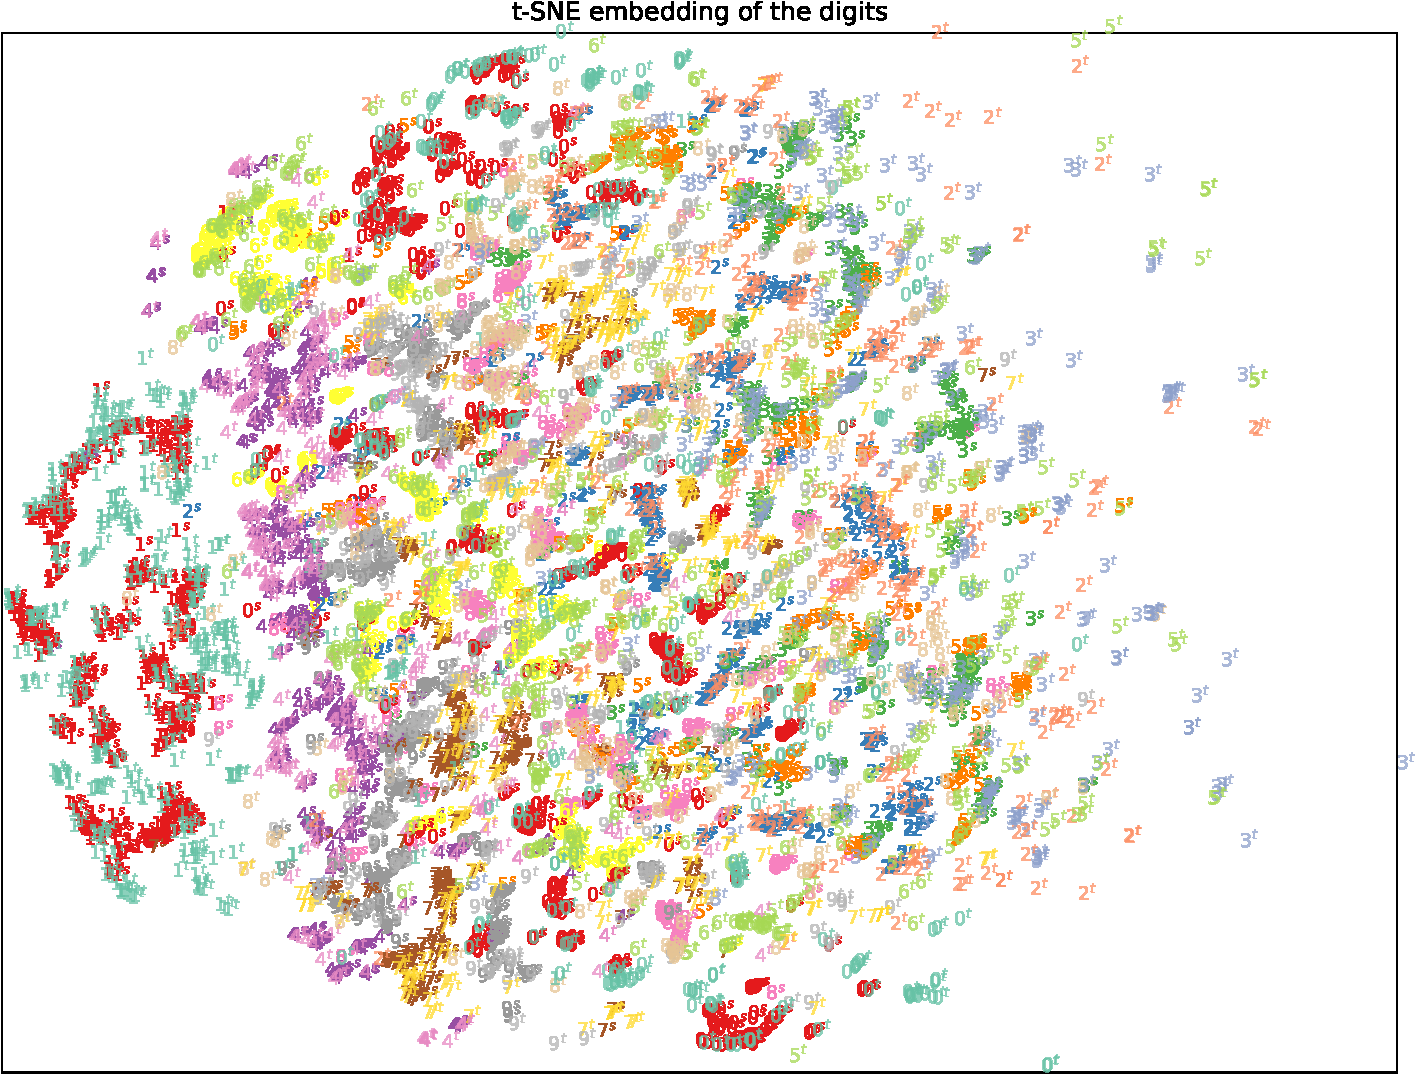
\includegraphics[width=0.7\linewidth]{figs/source-only-44300emb-st}
	\caption{Feature visualization of the Source-only method.}
	\label{fig:t-nse-s-only}
\end{figure}


\begin{figure}[h]
	\centering
	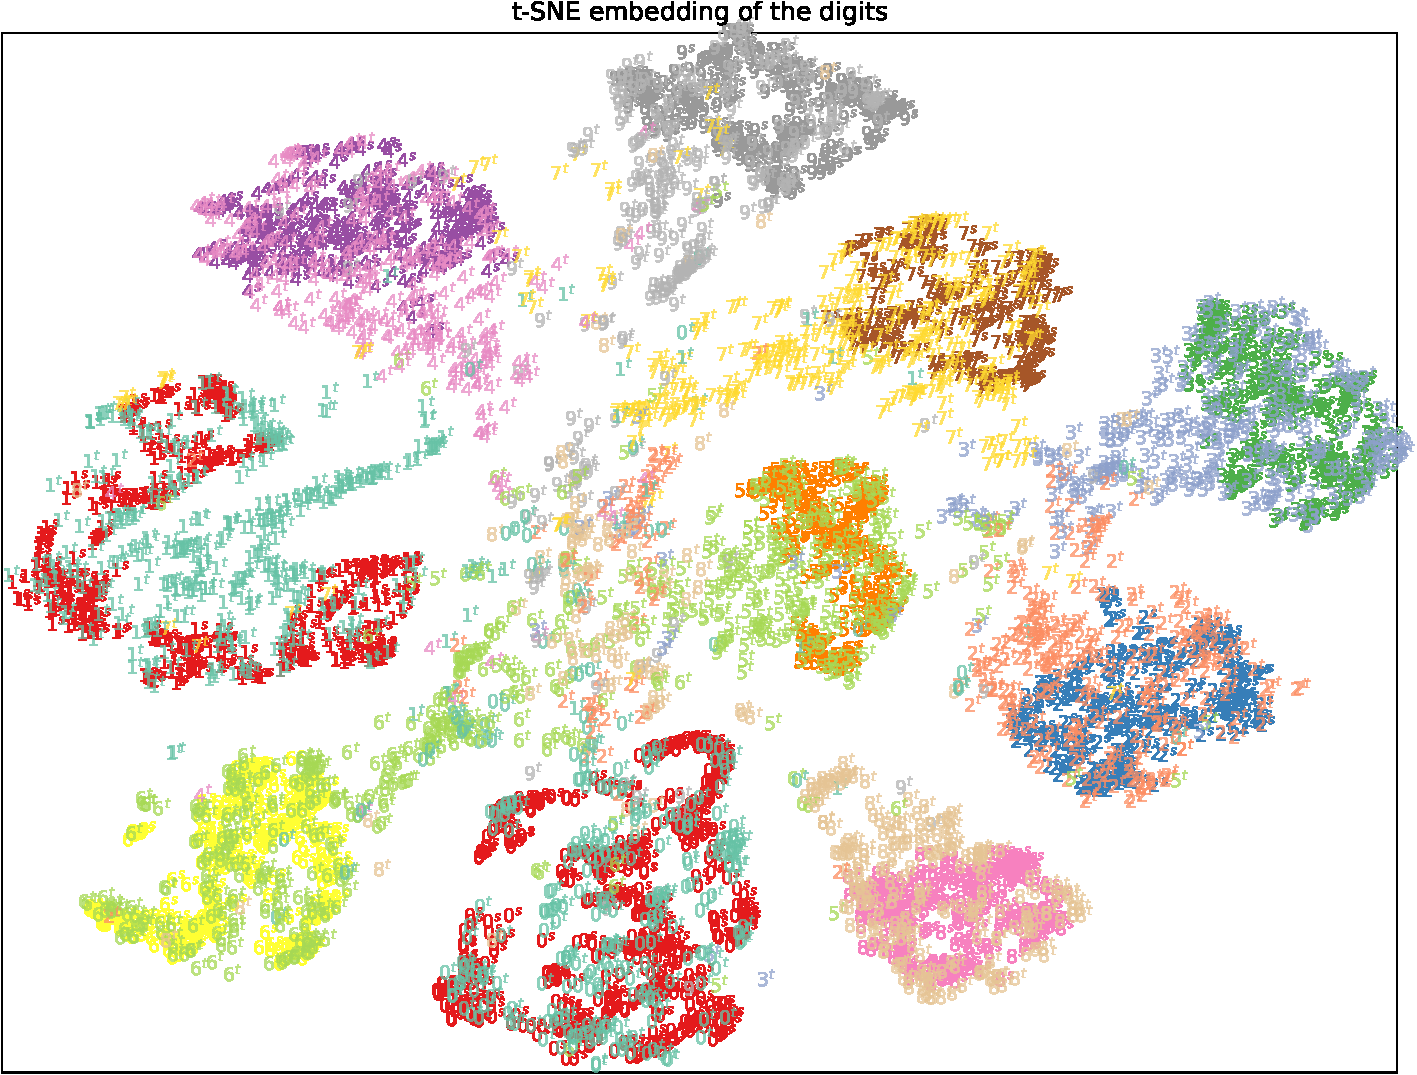
\includegraphics[width=0.7\linewidth]{figs/mmd-37000emb-st}
	\caption{Feature visualization of the MMD method.}
	\label{fig:t-nse-mmd}
\end{figure}

\begin{figure}[h]
	\centering
	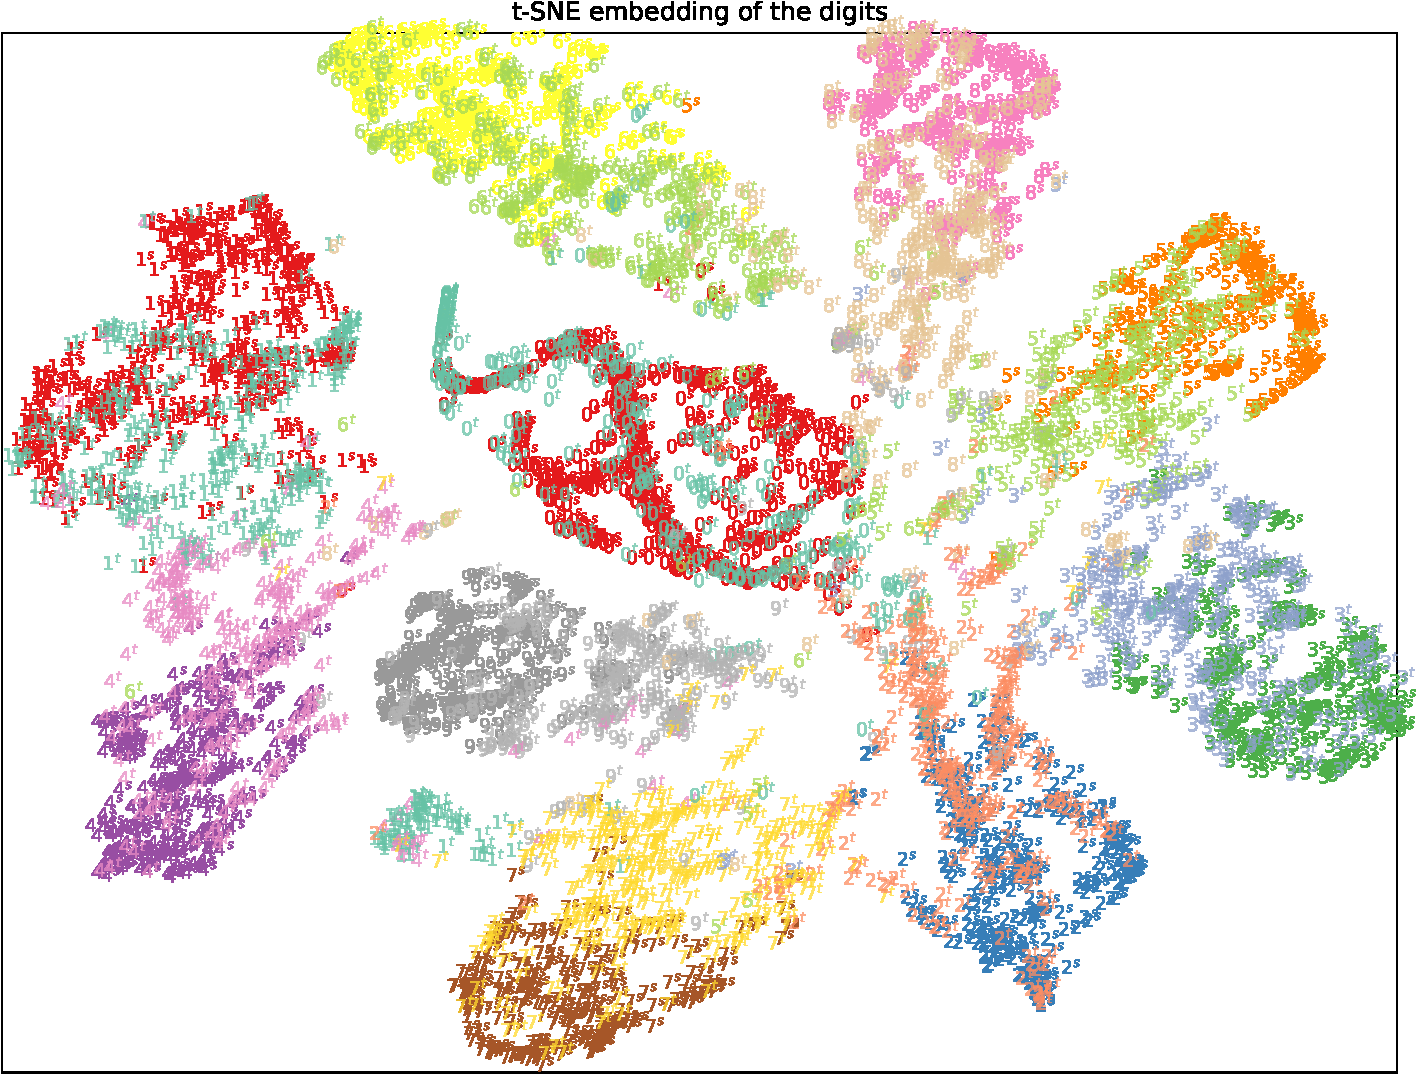
\includegraphics[width=0.7\linewidth]{figs/coral-47300emb-st}
	\caption{Feature visualization of the CORAL method.}
	\label{fig:t-nse-coral}
\end{figure}

\begin{figure}[h]
	\centering
	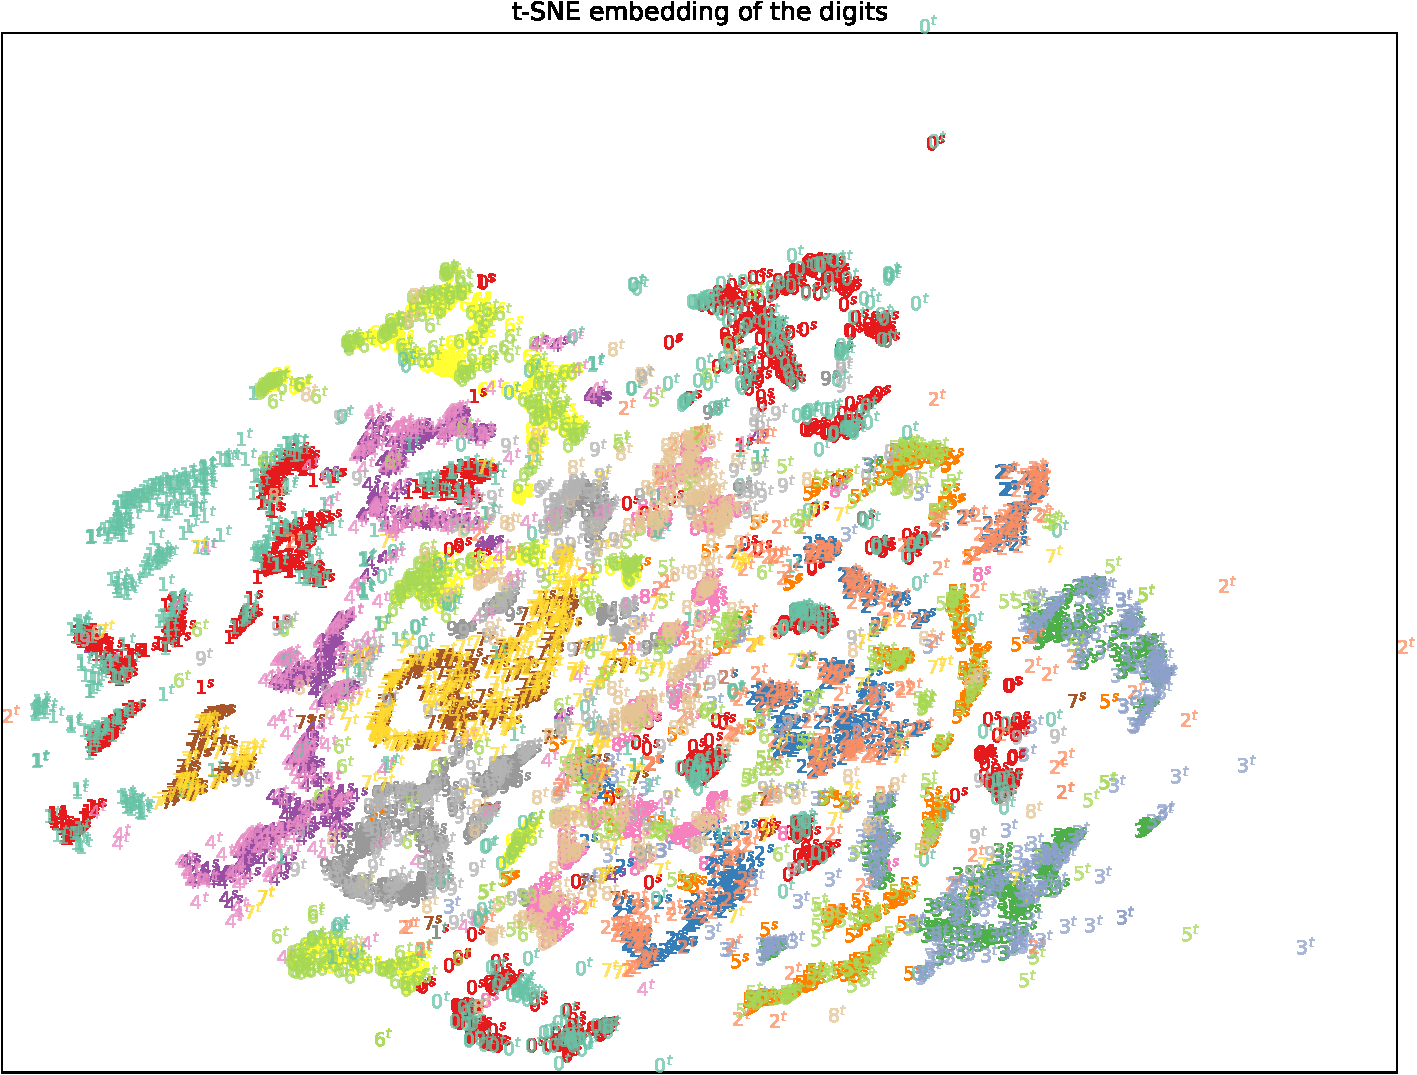
\includegraphics[width=0.7\linewidth]{figs/dann-36300emb-st}
	\caption{Feature visualization of the DANN method.}
	\label{fig:t-nse-dann}
\end{figure}

\begin{figure}[h]
	\centering
	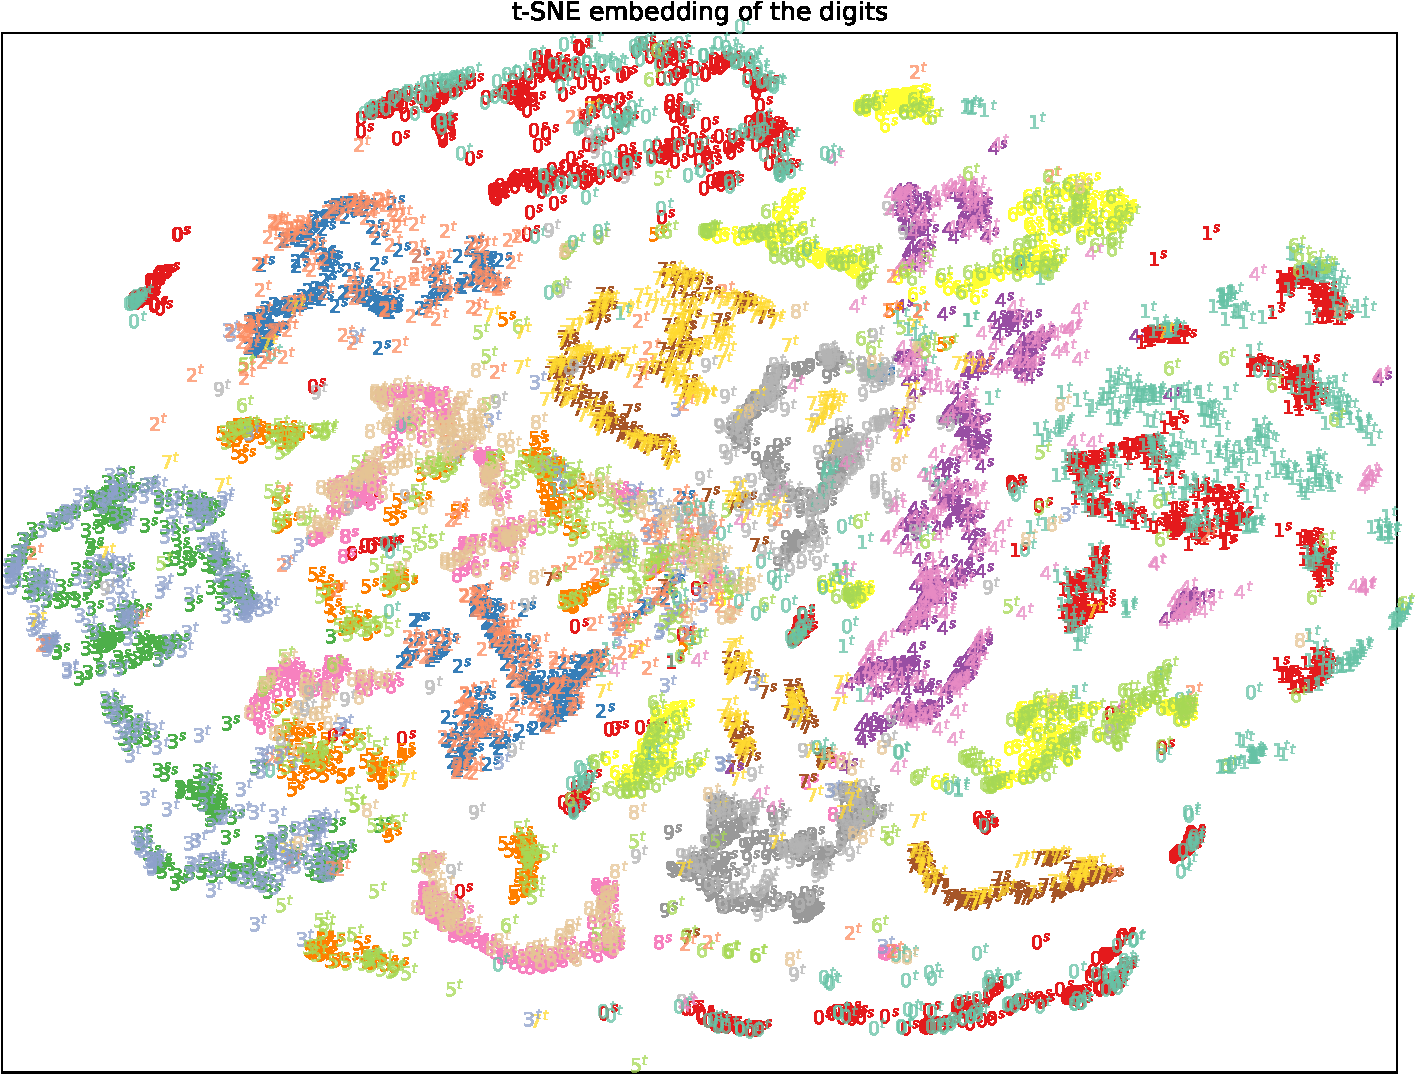
\includegraphics[width=0.7\linewidth]{figs/wd-20000emb-st}
	\caption{Feature visualization of the WDGRL method.}
	\label{fig:t-nse-wd}
\end{figure}

To have a better understanding of what happens during the training of domian adaptation, we plot the visualization of MMD at different stage during the training in Figure~\ref{ref:mmd-training}
\begin{figure}[h]
\centering
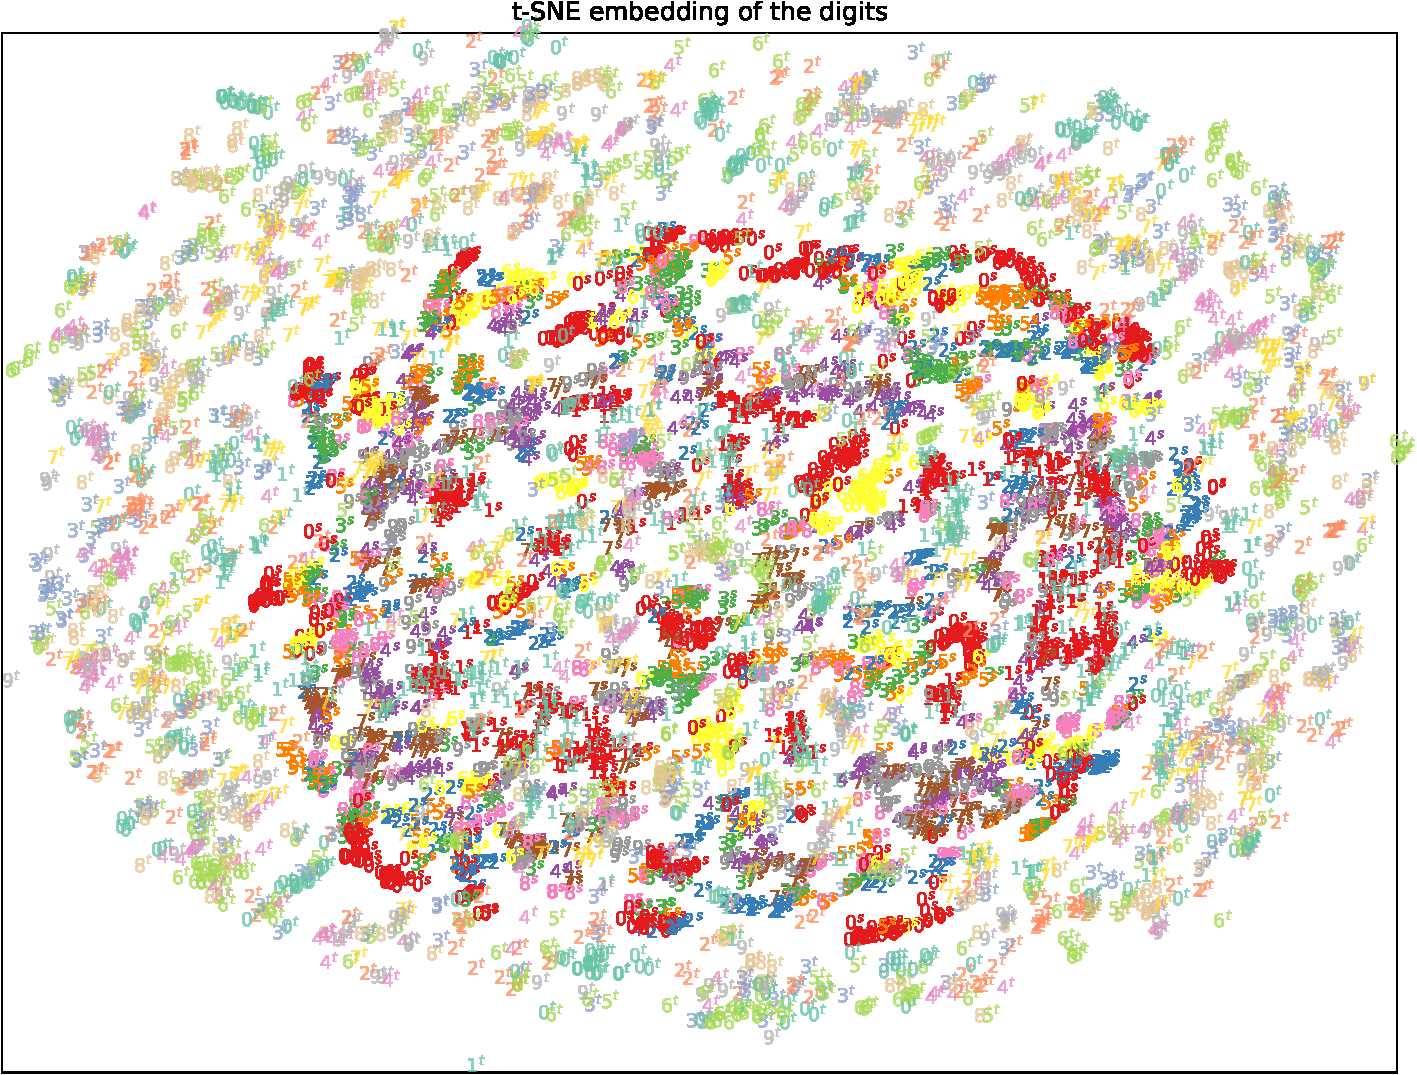
\includegraphics[width=0.32\linewidth]{figs/mmd-0emb-st}
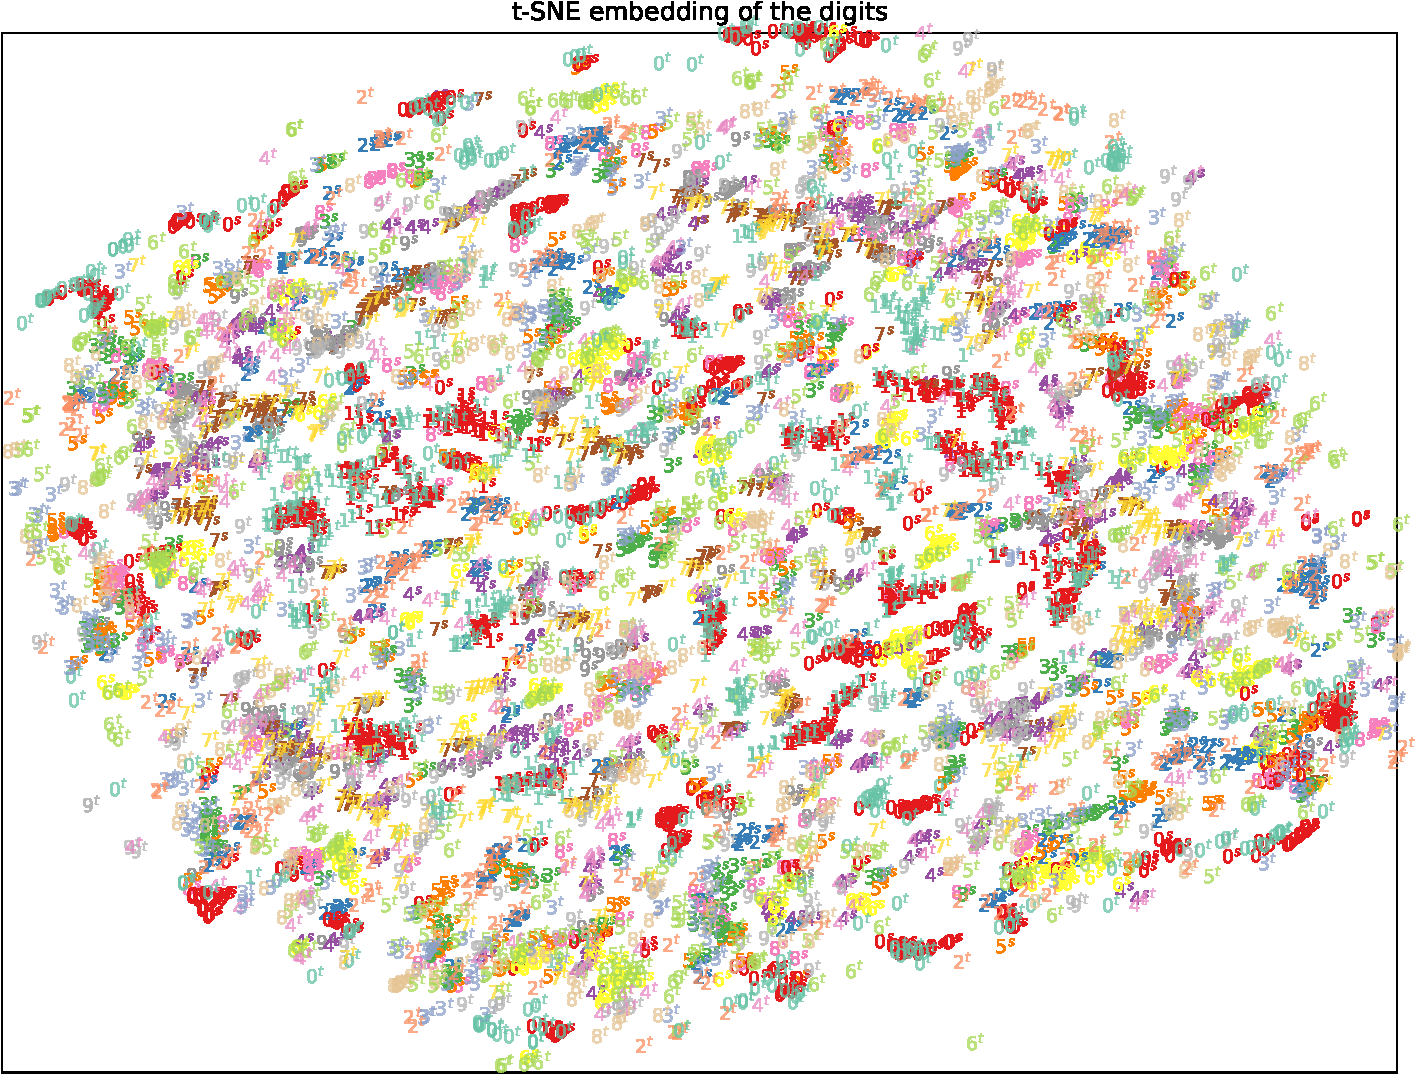
\includegraphics[width=0.32\linewidth]{figs/mmd-900emb-st}
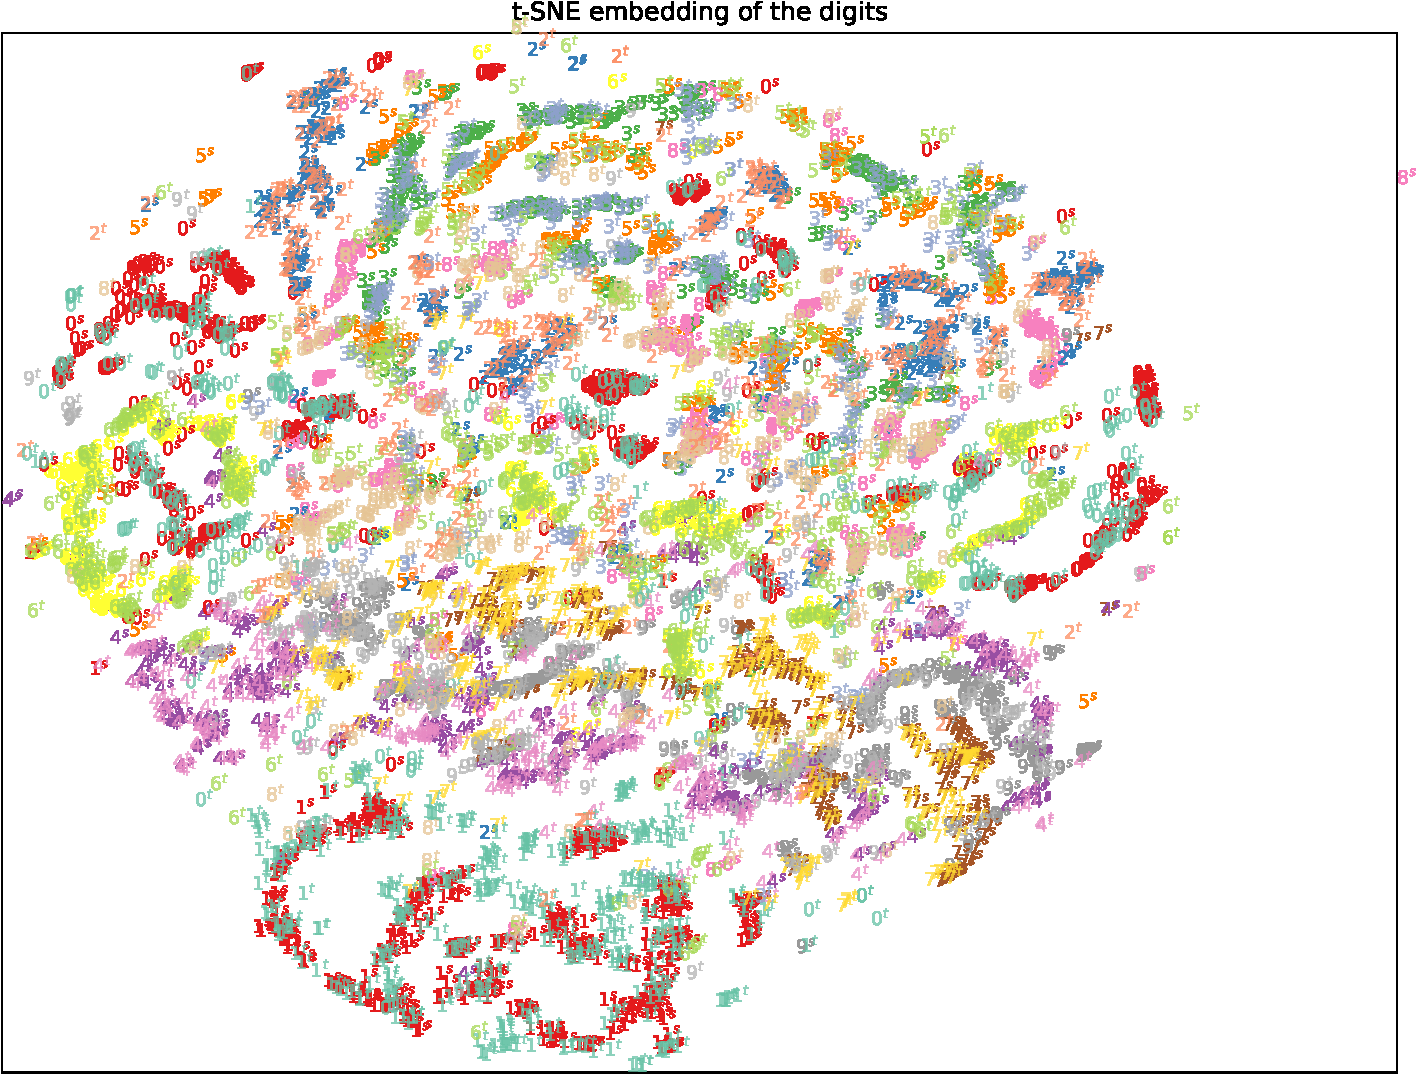
\includegraphics[width=0.32\linewidth]{figs/mmd-9900emb-st}
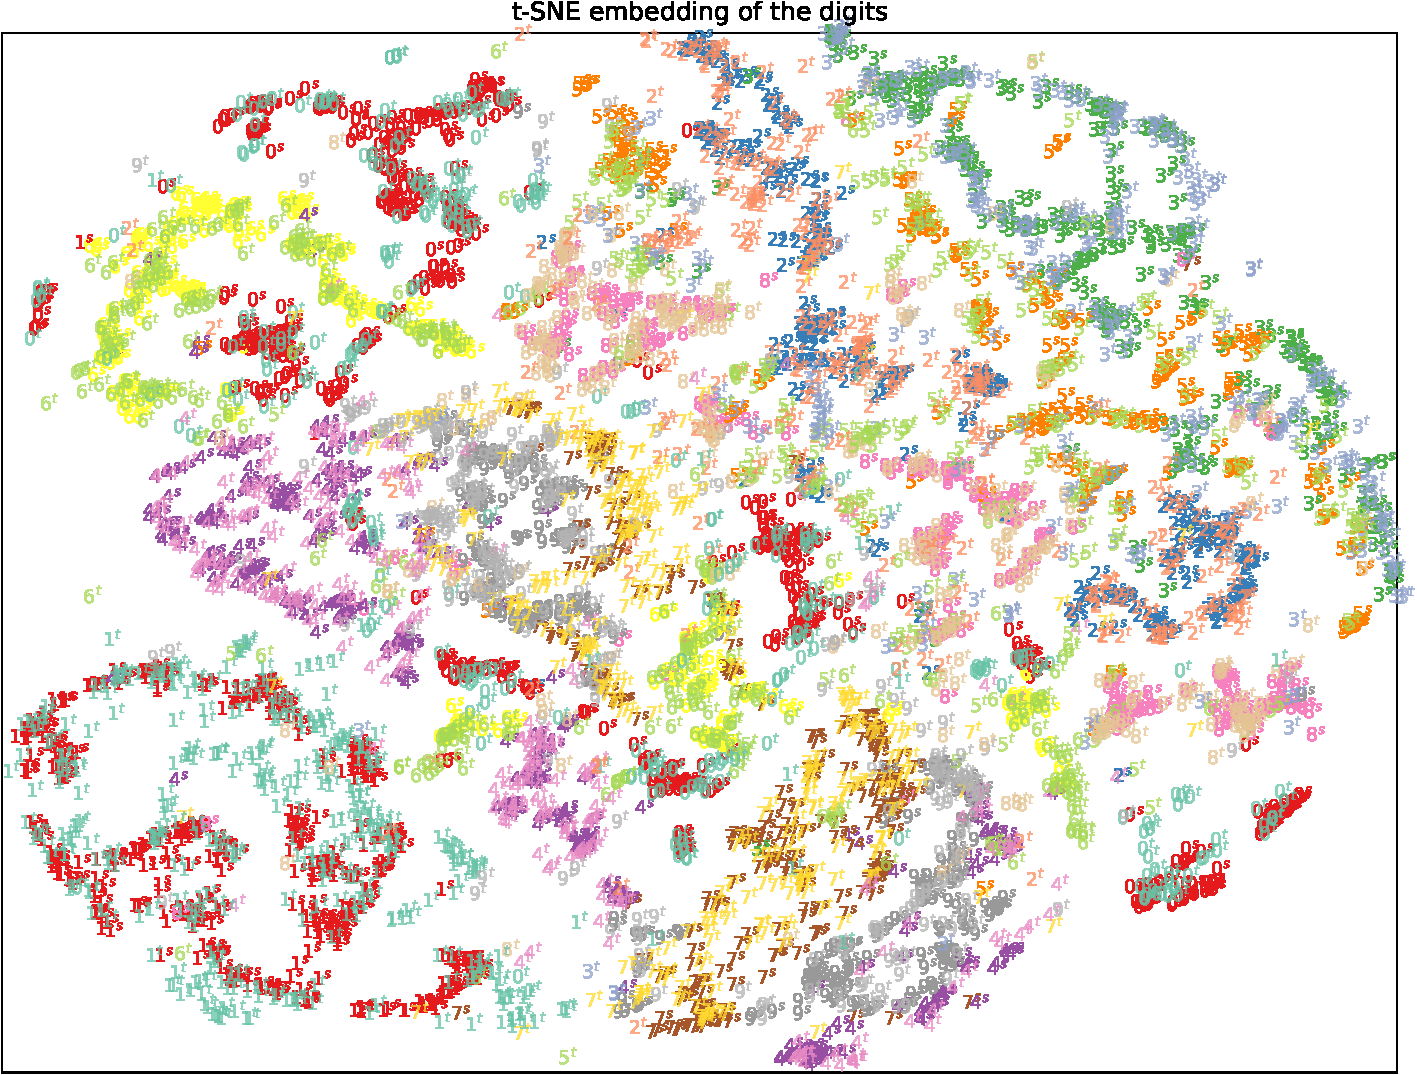
\includegraphics[width=0.32\linewidth]{figs/mmd-14600emb-st}
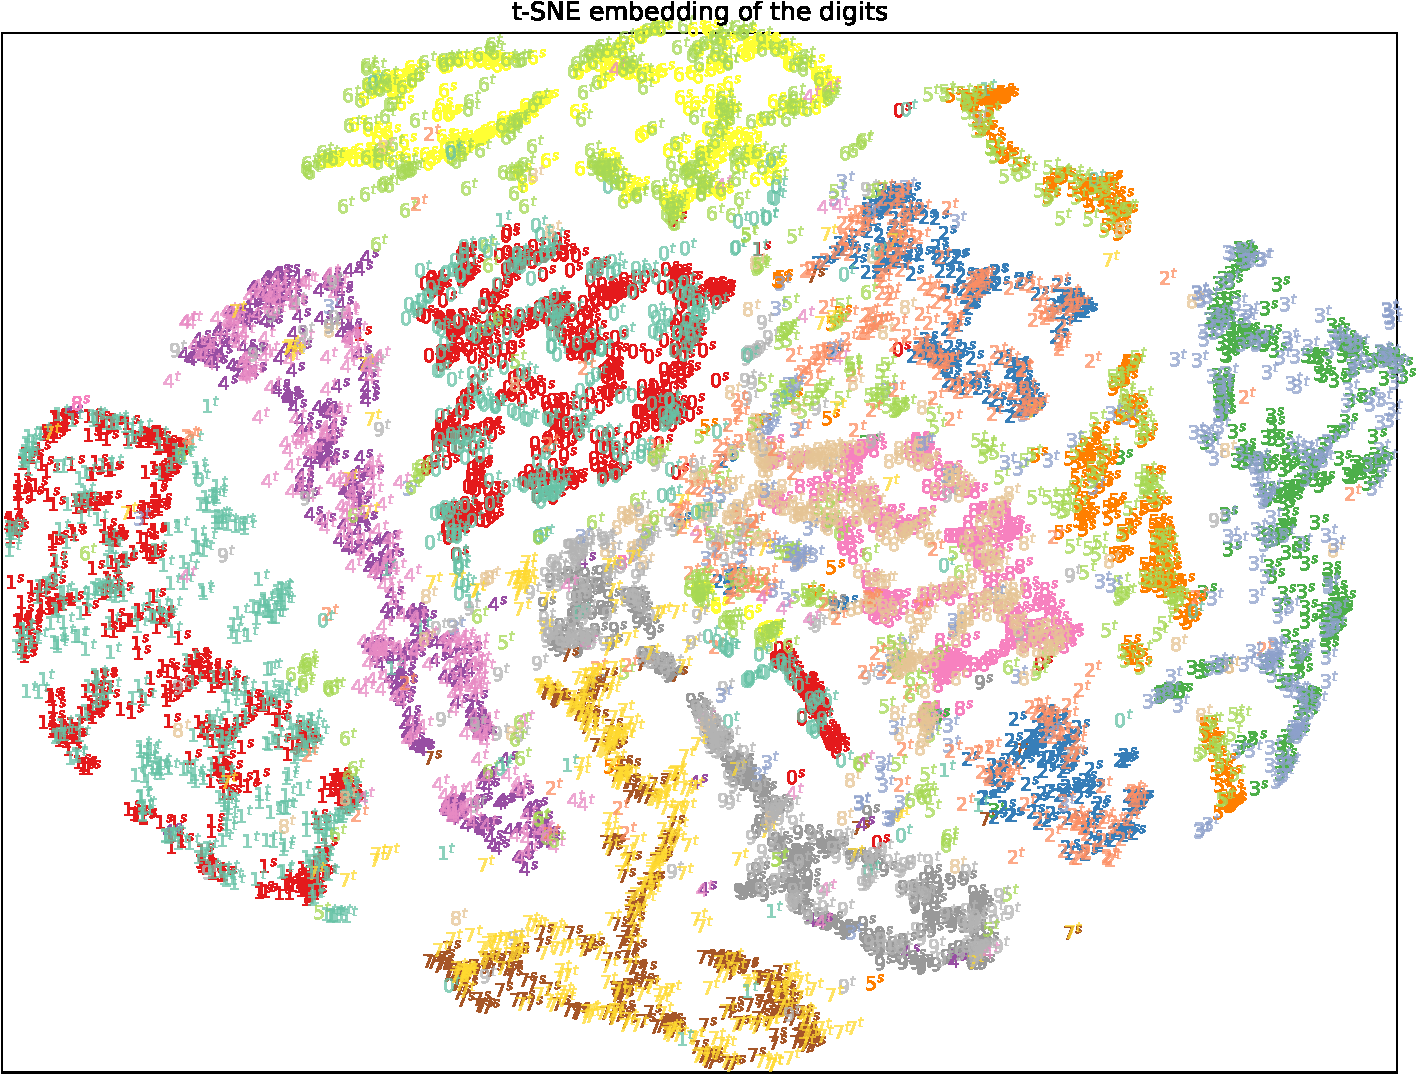
\includegraphics[width=0.32\linewidth]{figs/mmd-17700emb-st}
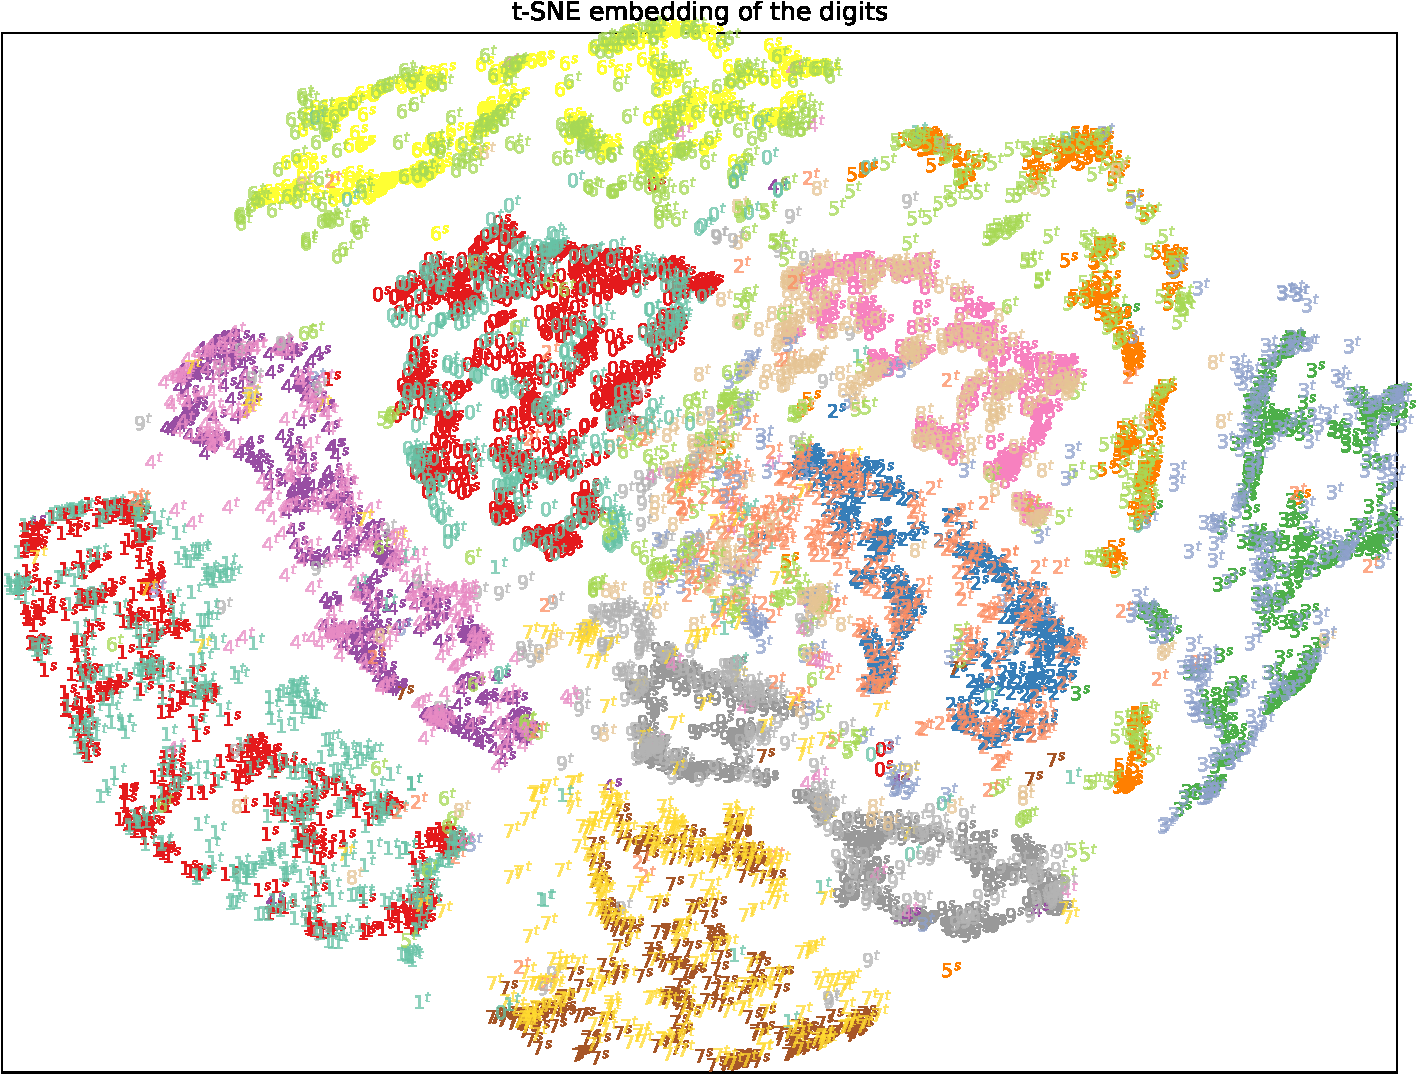
\includegraphics[width=0.32\linewidth]{figs/mmd-18300emb-st}
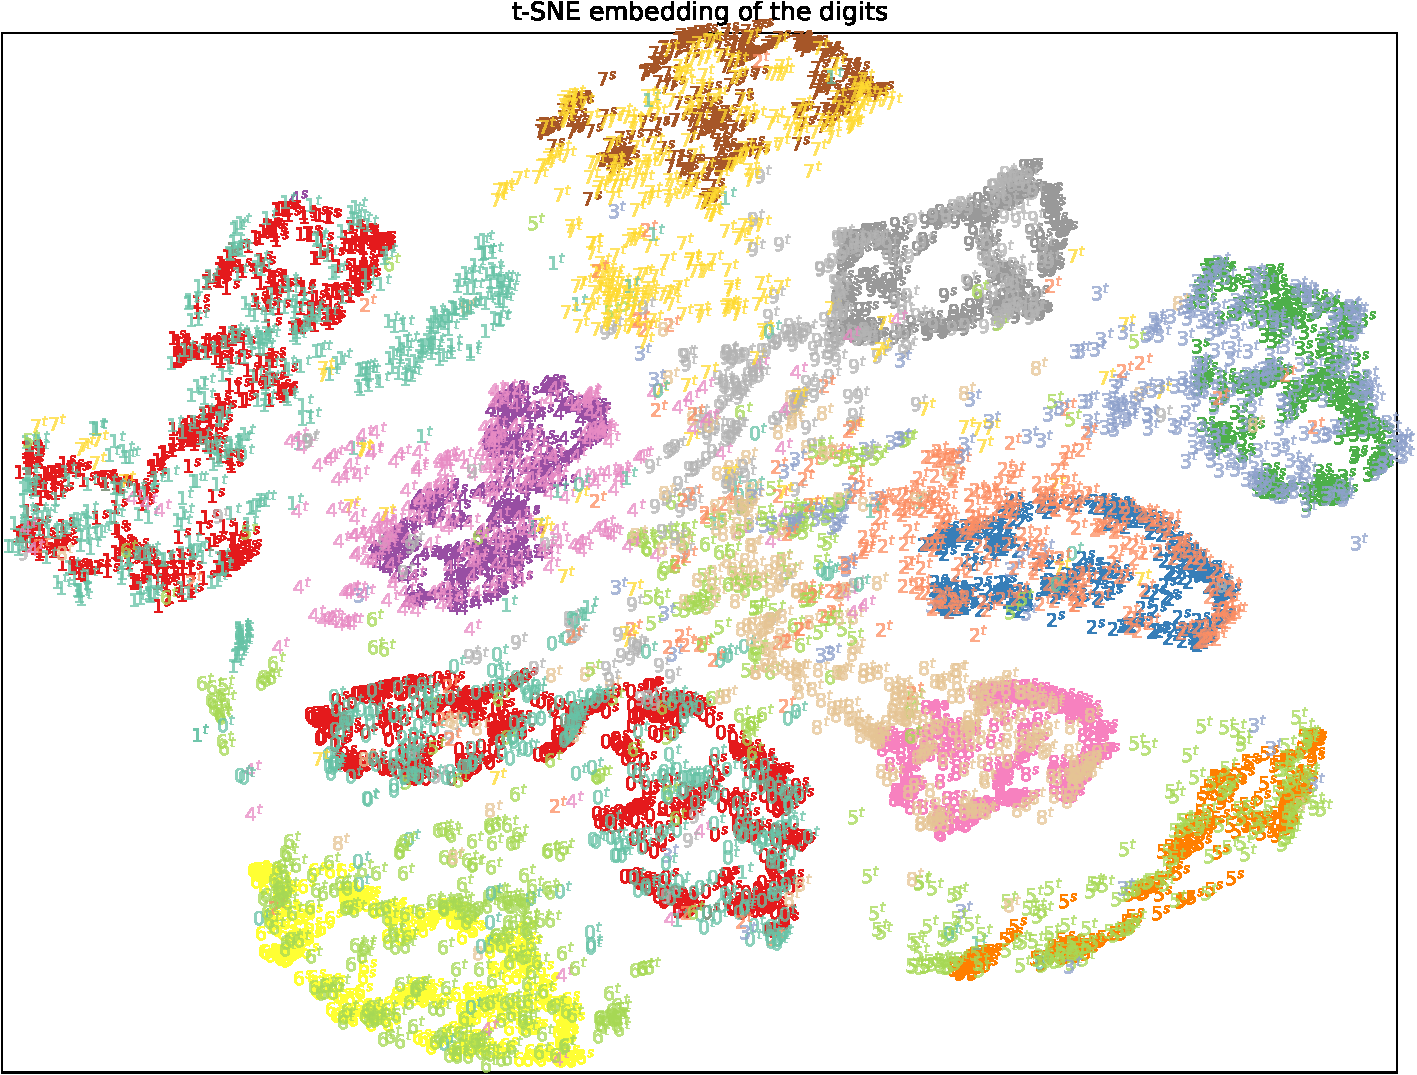
\includegraphics[width=0.32\linewidth]{figs/mmd-26700emb-st}
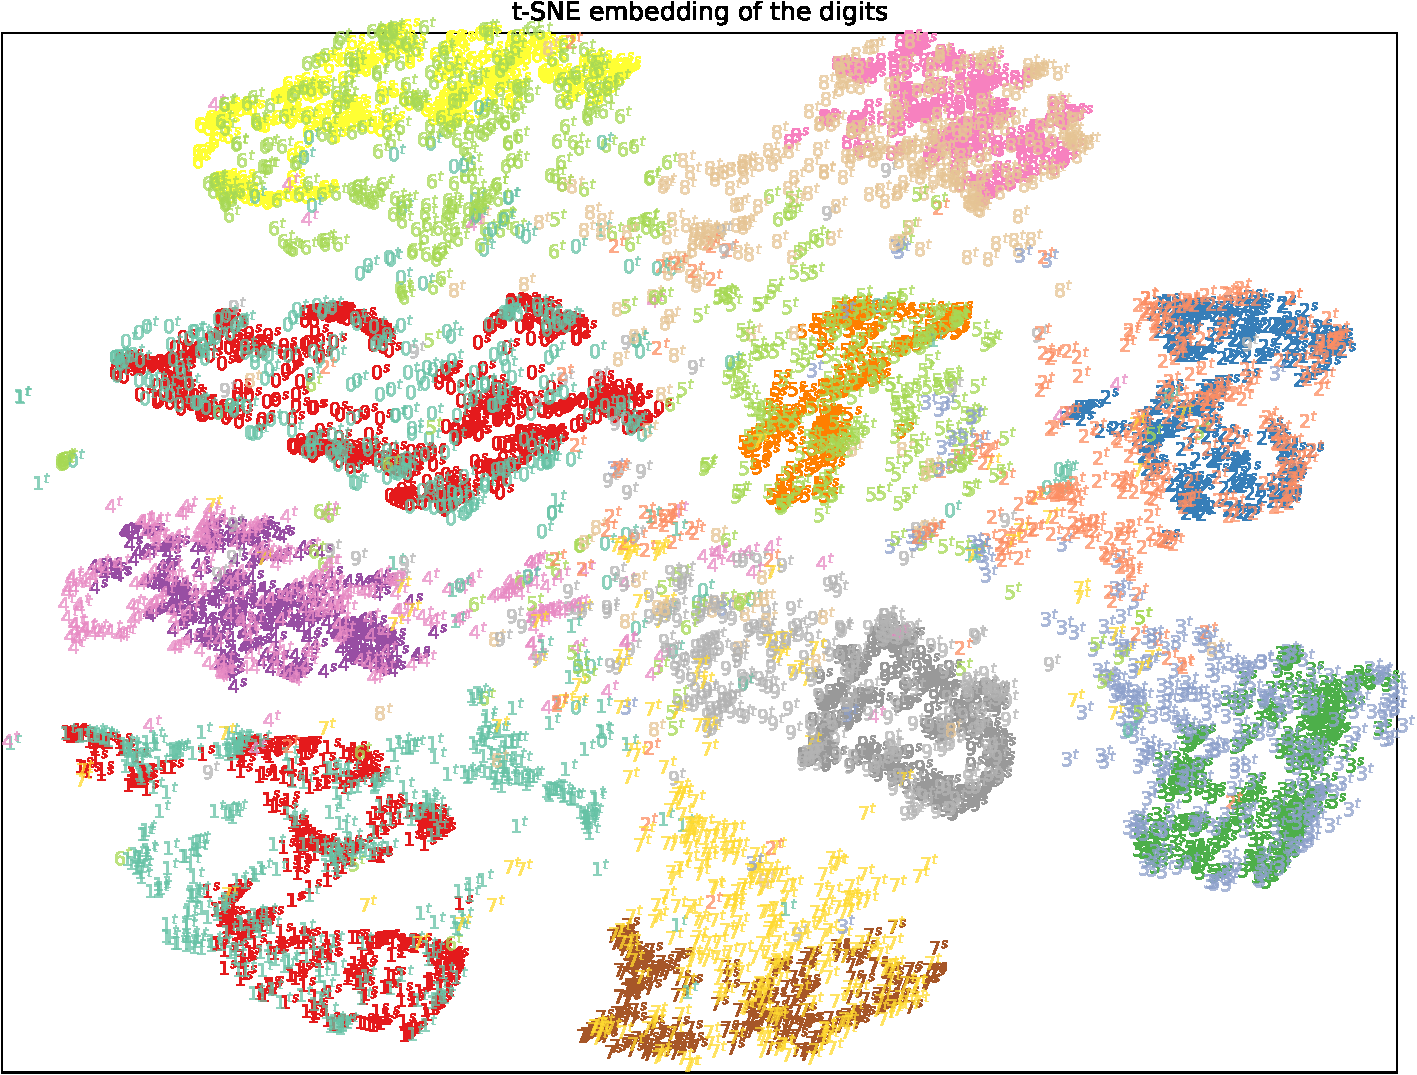
\includegraphics[width=0.32\linewidth]{figs/mmd-32700emb-st}
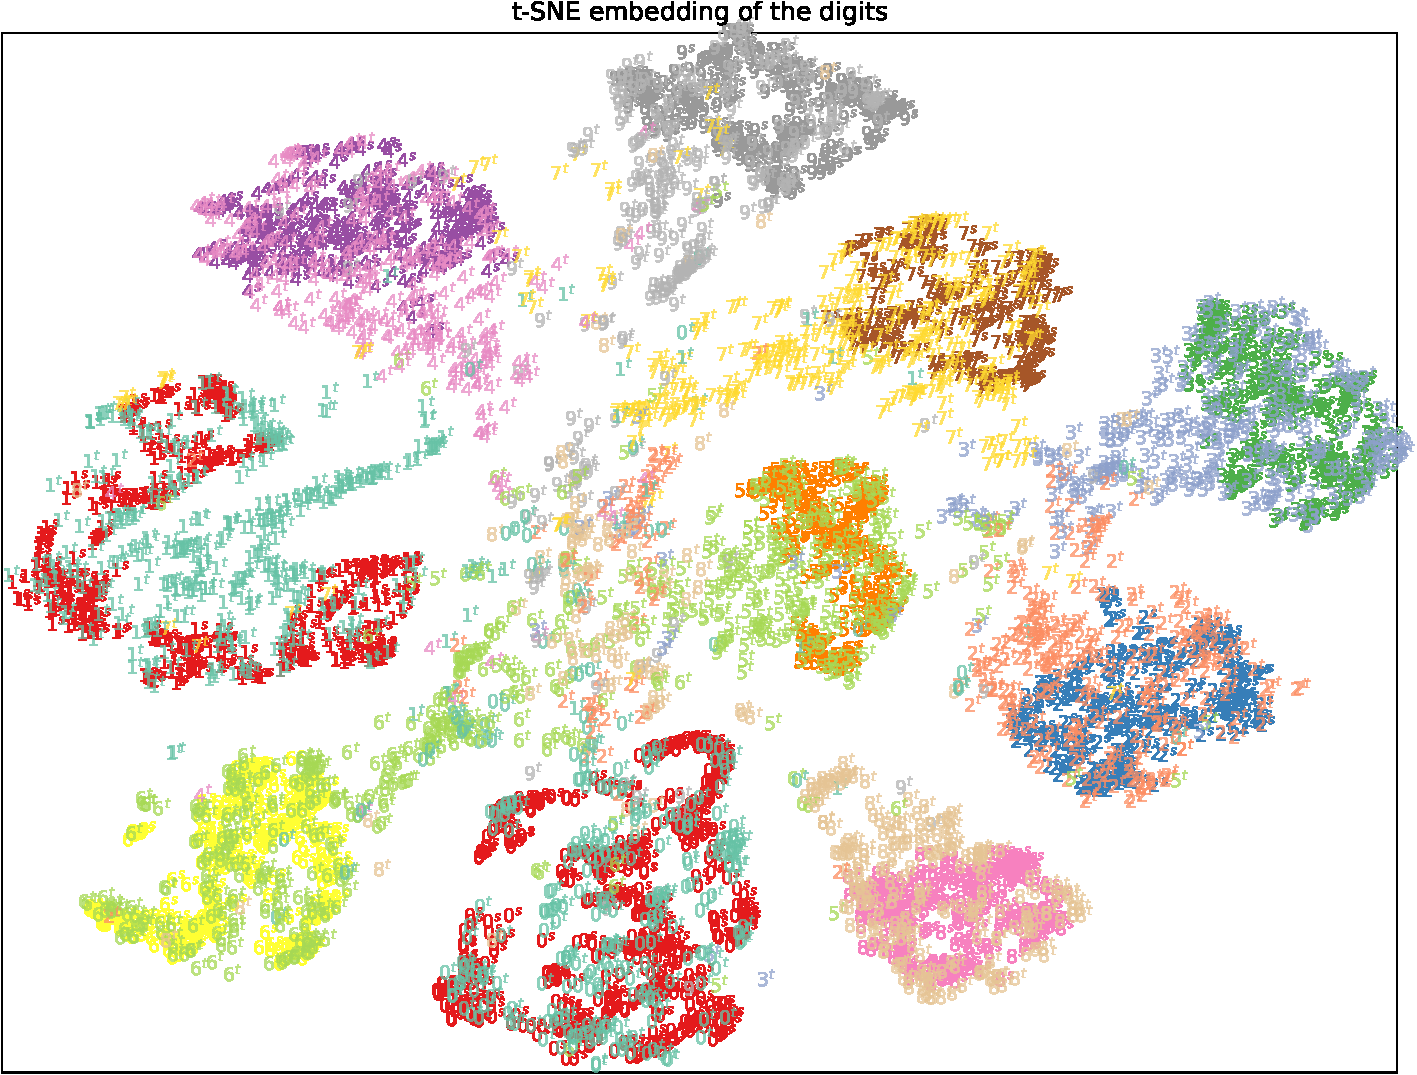
\includegraphics[width=0.32\linewidth]{figs/mmd-37000emb-st}

\caption{Visualization of MMD method during training.}
\label{ref:mmd-training}
\end{figure}
We can find that, at the very beginning, the distribution of source and target domain are totally different (the first subfigure). after some training of MMD, in the second subfigure, the distribution is some how closer, at least, they are mixed together, but not separated as the very beginning. In the third one, we can see that there are some clusters now. This means the network begins to learn some meaningful representations. And more importantly, the representations of the some digits from source and target domain are clustered together. The MMD works!  Then in the 4-8 subfigure, the ten clusters are becoming more and more clear. And in each cluster, there are one kind of digit from both source and target domain. And finally in the last subfigure, we get the final representation of the digit. The distribution of source and target domain are quite similar, thus the classifier with high-performance on source domain can perform well on target domain. But we must note that a small amount of target domain digits are still mixed in the middle, these digits might be the reason why we still has a performance gap between source and target domain. And also, there is some room for improvement. 


\section*{Conclusion}
In this paper, several models have been implemented studied for the MNIST classification task, i) CNN, ii) Capsule Network, iii) deep forest. Extensive experiments show the effectiveness of these methods. We also want to study how can we train a high-performance classifier with no label information on the modified MNIST dataset from a labeled source domain, which is called domain adaptation. We make our implementation available at \url{https://github.com/felixwzh/SJTU-CS420}.


\bibliographystyle{unsrt}
\bibliography{refs}
\end{document}
